%%%%%%%%%%%%%%%%%%%%%%%%%%%%%%%%%%%%%%%%%%%%%%%%%%%%%%%%%%%%%%%%%%%%%%%%%%%%%%%%
% reconstruction.tex:
%%%%%%%%%%%%%%%%%%%%%%%%%%%%%%%%%%%%%%%%%%%%%%%%%%%%%%%%%%%%%%%%%%%%%%%%%%%%%%%%
\chapter{Event Reconstruction and Selection}
\label{sec:reco_chapter}
%%%%%%%%%%%%%%%%%%%%%%%%%%%%%%%%%%%%%%%%%%%%%%%%%%%%%%%%%%%%%%%%%%%%%%%%%%%%%%%%

\WR decays produce electrons, muons, and jets that generate signals in multiple sub-detectors (Figure 
\ref{fig:particleTrajectories}).  In the data analysis, offline selection criteria are applied to select events that have two jets 
and two leptons whose kinematics are consistent with those of the \WR progeny.  The reconstruction algorithms, lepton triggers, and 
offline selection criteria are described in this section.

The reconstruction algorithms used in and the event selection criteria applied to data and simulated events, used to estimate the 
signal and the background, were identical.  In this section, any difference in reconstruction and selection efficiency between data 
and simulated events is described.

\begin{figure}[h]
	\centering
	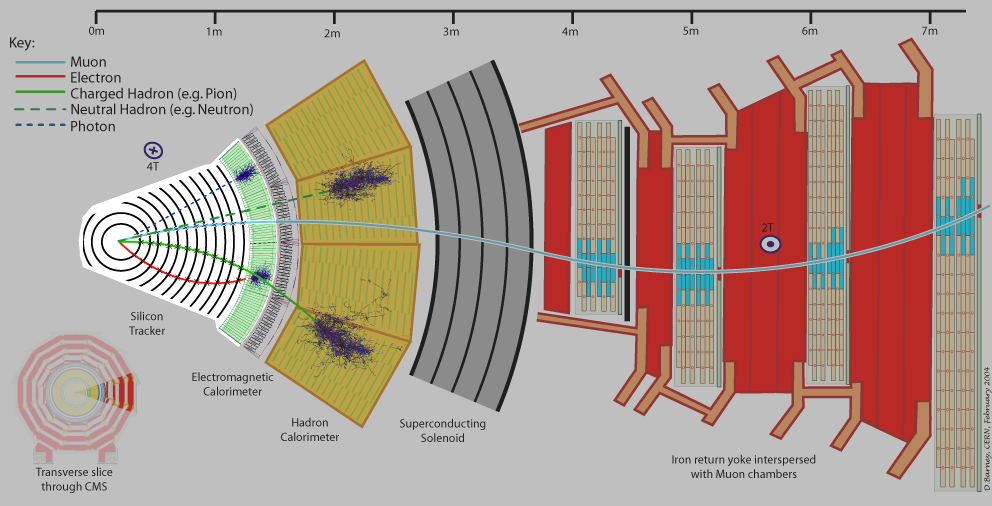
\includegraphics[width=0.75\textwidth]{figures/flowOfParticlesThroughCMS.png}
	\caption{Typical trajectories of particles travelling through CMS, from CERN.}
	\label{fig:particleTrajectories}
\end{figure}


\section{Track Reconstruction}
\label{sec:trkReco}
Muons and charged hadrons are reconstructed as helical tracks from signals measured in the silicon tracker and, in the case of muons, 
with the muon detectors.  A reconstruction algorithm starts by reconstructing tracks from signals found in the innermost pixel tracker 
layer that were closest to the IP.  After identifying track candidates in the innermost layer, 
the algorithm works radially outward, and builds longer track candidates by including new signals.  Signals in successive layers are 
linked and identified as tracks using a Kalman filter that requires each additional track point's measured position to be consistent with 
the track trajectory within $\chi^{2} <$ 30 \cite{trackerPerformanceInCollisions}.  Each time a new position measurement is added to 
a track, all the track parameters are recalculated, and an analytic function extrapolates the track trajectory to the next layer assuming energy 
can be lost through multiple scattering and ionization in the silicon.  Signals in the next layer are searched for in the region identified 
by this extrapolation.  This procedure is repeated out to the outermost silicon strip tracker layer.  Then, the same algorithm is applied 
in reverse - starting from the outermost strip layer and working inward - to identify track points that were missed and are compatible 
with an existing track.  Then, the track points that are linked into tracks are removed from the list of track candidates, and the algorithm 
is restarted using signals measured in the innermost pixel tracker layer that were further from the IP.  Using this algorithm, isolated muons 
with a $\pt > 0.9$ $\GeV$ and an $|\eta| < 2.4$ were reconstructed as tracks with essentially 100\% efficiency \cite{trackerPerformanceInCollisions}.  
After reconstructing all tracks in an event, each point where two or more tracks originate is identified as an interaction vertex.  A vertex 
is required to have at least two reconstructed tracks originating within 2 mm of the vertex position.  The positions of vertices that have muon 
tracks with $|\eta| < 1.4$ and $\pt = 100$ $\GeV$ were measured with 10 and 30 $\mu$m resolutions in the transverse (r-$\phi$) and longitudinal ($z$) directions.

Using a second track reconstruction algorithm, electrons are reconstructed as helical tracks from signals measured in the silicon 
tracker.  This is necessary because the tracker contains 1 to 2 radiation lengths of material, causing electrons to 
shower and lose energy through bremsstrahlung.  The electron track reconstruction algorithm uses the same iterative track reconstruction procedure 
described previously, but extrapolates each track's trajectory to the next silicon layer assuming the track loses energy through bremsstrahlung 
that is described by a sum of six Gaussians \cite{gsfFunction}.  The Gaussian widths can be any positive value, but their total width 
must minimize the difference in the cumulative probability function of the predicted energy loss between the Bethe-Heitler formula 
and the six-Gaussian approximation.  Also, the Kalman filter used to link signals in successive layers requires that additional signals 
need to have $\chi^{2} <$ 2000.  Using the electron track reconstruction algorithm, electrons that had $\pt > 20$ $\GeV$ and were within 
$|\eta| < 2.5$ were reconstructed as tracks with an efficiency $\geq$ 97\% \cite{gsfPerformanceInCollisions}.

\subsection{Muon Reconstruction}
\label{sec:muReco}
Muons are reconstructed as tracks from signals measured in individual muon chambers.  In each DT chamber, the start 
and end points of track candidates are identified as pairs of track points measured in the same plane (r-$\phi$ or r-z) but in different 
layers.  Then, straight lines representing the track candidates are drawn between the pairs of points, and candidates that do not project 
to the IP are discarded.  The trajectories of these candidates are compared to the positions of all track points, and the points that 
overlap with the candidate trajectories are merged with the candidates to build track segments that are measured in at least 3 layers.  
In each plane the track segment that is measured in the largest number of layers ($N_{layer}$) and has the lowest $\chi^{2}/nDOF$ 
($\chi^{2}_{min}$), less than 20, is used to build a 3D track.  If there are two or more track segments in one plane with the same 
$N_{layer}$ and $\chi^{2}_{min}$, then all combinations of r-$\phi$ and r-z track segments are used to build tracks.  In practice, only 
$\sim$1\% of events have more than 1 track in a DT chamber \cite{cmsTdrPhysPerformance}.  The same track segment reconstruction algorithm 
is used in each of the six-layer, single plane CSCs.  There, the final track segment is required to have signals in at least 4 layers.  
In the barrel-endcap transition region ($1.3 < |\eta| < 1.6$) where the DT chambers end and the CSCs begin, RPCs 
are used to improve the muon reconstruction efficiency and the precision of arrival time measurements.  Each RPC contains two parallel 
plates divided into many thin strips, and strips that measure a signal are grouped into clusters.  Each reconstructed cluster represents 
a hit whose position is the center of gravity of all the strips in the cluster.

Tracks in individual chambers are connected to reconstruct muon trajectories over several meters.  
A Kalman filter algorithm similar to the one used to reconstruct electron tracks starts with tracks in the chambers closest to the IP, 
and predicts the track positions in chambers in the next 
radial station with the effects of an inhomogeneous magnetic field and material losses taken into account \cite{muonRecoFirstCollisions}.  
Track segments in outer chambers are added to existing tracks subject to a $\chi^{2}$ requirement, and existing tracks are propagated to 
the next radial station even if no matching track segment is found in the current station.  Once the outermost station is included, a 
reverse Kalman filter is applied to reconstructed tracks from the outermost to the innermost station.  The reverse Kalman filter is used 
to determine the final track parameters, and the resultant tracks are compared to tracks found in the silicon detector to identify muons.

Each silicon detector track that passes within 3 cm of a muon detector track is identified as a muon.  If a muon detector track has multiple 
silicon detector track candidates within 3 cm, the closest match is identified as a muon; and comparing the results of the silicon detector 
track and the muon detector track determines the $(\eta,\phi)$ trajectory of each muon.

As there are two independent detectors each measuring the muon's momentum, four different muon reconstruction algorithms are composed, 
and the highest quality result is selected.  Each algorithm fits a continuous track \cite{cmsMuonRecoRunTwo} to a unique combination of 
silicon tracker and muon detector measurements to estimate a muon's trajectory, depicted in Figure \ref{fig:particleTrajectories}.  The 
quality of each continuous track is identified by a fit uncertainty $\chi^{2}/nDOF$ and momentum uncertainty $\sigma(\pt)/\pt$.  The 
track with the lowest $\chi^{2}/nDOF$ and momentum uncertainty $\sigma(\pt)/\pt < 0.3$ determines the muon's momentum.  
For muons with $\pt \lesssim 100$ $\GeV$ the highest quality result is obtained using only silicon tracker measurements.  Muons that had 
$|\eta| < 1.4$ and $\pt = 100$ $\GeV$ were measured with a $\pt$ resolution of $\sim$2.8\% \cite{trackerPerformanceInCollisions}.  
As a muon's $\pt$ increases above 100 $\GeV$ the silicon tracker $\pt$ resolution degrades faster that that of the muon 
detectors.  A significant fraction of $\WR \rightarrow \mu\mu jj$ events are expected to produce at least one muon with $\pt > 200$ $\GeV$ 
(Table \ref{tab:wrHighPtMuons}).  In this high $\pt$ region the highest quality momentum measurement comes from a combination of the 
silicon tracker and muon detector measurements, such that muons with $|\eta| < 0.9$ and $200 < \pt < 400$ $\GeV$ were measured 
with a $\pt$ resolution of 3.2\%; higher $\pt$ muons were measured with a resolution better than 6\% \cite{cmsMuonRecoRunTwo}.

\begin{table}[h]
	\caption{Fraction of expected $\WR \rightarrow \mu\mu jj$ events that had at least one muon with $\pt > 200$ $\GeV$. 
	($\mnul = \frac{1}{2}\mWR$)}
	\label{tab:wrHighPtMuons}
	\centering
	\begin{tabular}{c|c}
		\mWR ($\TeV$) & Fraction of events with at least one high-$\pt$ muon (\%) \\  \hline
		1.0 &  80.  \\
		2.0 &  95.  \\ 
		3.0 &  98.  \\ \hline
	\end{tabular}
\end{table}

Muons produced in simulated events are reconstructed with a higher efficiency than muons produced in real collisions.  This efficiency 
difference was corrected by multiplying the weight of each simulated event by a value between 0.99 (1\% decrease) and 1.0, depending on 
the muon $\pt$ and $\eta$, for each muon that was selected.


\section{Energy Measurement}
\label{sec:enrgReco}
The energies of photons and electrons are measured in groups of ECAL crystals.  Photons and electrons 
impinging on the ECAL generate signals in the ECAL crystals that are converted into uncalibrated energies.  The most energetic crystals 
with $\Et \gtrsim 0.2$ $\GeV$ and their nearest neighbors are grouped into superclusters (SCs) that are at least 3 crystals wide in 
$\eta$.  The upstream tracker material causes $\sim$35\% of electrons and photons to shower early in the tracker 
\cite{trackerPerformanceInCollisions}, and the magnetic field spreads the shower over several crystals in $\phi$.  To capture the early 
shower energy, each SC is at least 5 crystals wide in $\phi$, and can be much larger, as in Figure \ref{fig:eleTrackAndSC}.  Once a SC 
is built, the energy of each crystal in the SC is multiplied by a laser transparency correction, and relative and absolute energy 
calibration corrections.  The sum of the calibrated crystal energies is the SC energy, and the energy weighted average $(\eta,\phi)$ 
position is the SC position.  Using only ECAL SCs, the $(\eta,\phi)$ positions of electrons in the barrel (endcap) were measured with 
a $\phi$ resolution of 0.17$^{\circ}$ (0.29$^{\circ}$), and an $\eta$ resolution of 0.001 (0.002) units.

The energies of hadrons are measured over 10 nuclear interaction lengths of material, the first of which is the lead tungstate ECAL.  
Up to 25\% of hadrons start showering in the tracker \cite{trackerPerformanceInCollisions}, so hadrons impinging on the ECAL are 
reconstructed as SCs like electrons and photons.  Hadrons impinging on the HCAL generate 
signals in the HCAL towers that are converted into uncalibrated energies.  The highest energy towers with $\Et \gtrsim 1$ $\GeV$ are 
used to seed tower clusters, which include all neighboring towers that have $\Et > 0.8$ $\GeV$ \cite{pflowEventReco}.  If one tower is 
grouped into multiple clusters, the tower's contribution to each cluster is weighted by its distance from each cluster's seed.  After 
the clusters are built, each tower's energy is multiplied by a laser transparency correction, and relative and absolute energy calibration 
corrections.  The sum of the calibrated tower energies is the cluster energy, and the energy weighted average $(\eta,\phi)$ position is 
the cluster position.  Combining ECAL and HCAL energy measurements, hadrons that have $\Et = 100$ $\GeV$ were measured with a resolution 
of 10\% $\Et$ \cite{pflowEventReco}.

\subsection{Electron, Photon, and Hadron Reconstruction}
\label{sec:elePhoHadReco}
A track is identified as being caused by an electron if it extrapolates from the outermost silicon strip layer to the front face of the 
ECAL, and matches a shower found at that location, represented by an ECAL SC.  If a track matches the $(\eta,\phi)$ position of a SC to 
within 1.0$^{\circ}$ (1 crystal wide) in $\phi$ and within 0.004 units (below $\frac{1}{2}$ a crystal wide) in $\eta$, then 
the track and ECAL SC are identified as an electron candidate.  If the measured $\Et$ and the matched track $\pt$ agree within the track 
$\pt$ uncertainty, then the track and shower are identified as being caused by an electron.  Using the SC energy, electrons with 
$\Et \approx 45$ $\GeV$ and $|\eta| < 0.8$ were measured with an $\Et$ resolution better than 2\%, and a resolution between 2\% and 5\% 
at higher values of $|\eta|$ \cite{ecalPerformanceInCollisions}.

\begin{figure}[h]
	\centering
	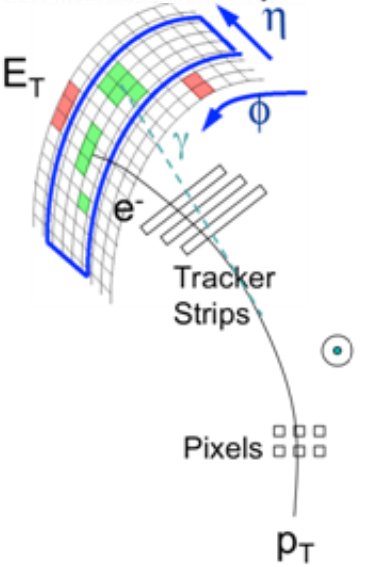
\includegraphics[width=0.3\textwidth]{figures/electronTrackAndSupercluster.png}
	\caption{The trajectory of a typical electron through the tracker and the ECAL.}
	\label{fig:eleTrackAndSC}
\end{figure}

Electrons produced in simulated events are reconstructed with a higher efficiency than electrons produced in real collisions.  This 
efficiency difference was corrected by multiplying the weight of each simulated event by 0.982 for each electron that was selected.

After electrons have been identified, ECAL SCs are identified as being caused by photons using the remaining reconstructed tracks.  A SC 
that does not match any reconstructed track within the matching window ($\Delta \eta =$ 0.004 units, $\Delta \phi =$ 1.0$^{\circ}$) is 
identified as a photon.  Alternatively, an ECAL shower that matches a reconstructed track within the matching window is identified as a 
photon if its $\Et$ does not agree with the track $\pt$ within the uncertainty of the measurement of the track $\pt$.

A reconstructed track is identified as being caused by a charged hadron using the calorimeter energy clusters.  A track that is not 
identified as an electron is extrapolated from the outermost silicon strip layer to the HCAL front face, and its $(\eta,\phi)$ position is 
compared to that of the HCAL clusters.  If a track intersects any portion of an HCAL cluster, and the cluster $\Et$ and track $\pt$ agree 
within the $\Et$ uncertainty, then the track is identified as being caused by a charged hadron.  The track $\pt$ and $(\eta,\phi)$ 
determine the charged hadron kinematics.

After all charged tracks have been identified as leptons or hadrons, an HCAL cluster that is not intersected by a track is identified as 
a neutral hadron.  Also, an HCAL cluster that is intersected by a track is identified as a neutral hadron if its $\Et$ 
does not agree with the track $\pt$ within the uncertainty of the measurement of the $\Et$.  If an ECAL SC (energy $E_{ECAL}$, 
uncertainty $\delta E_{ECAL}$) overlaps with any portion of an HCAL cluster (energy $E_{HCAL}$, uncertainty $\delta E_{HCAL}$) identified 
as being caused by a neutral hadron, then the SC can be identified as coming from a neutral hadron.  The SC is identified as a neutral 
hadron if $E_{ECAL}$ and $E_{HCAL}$ agree within the larger of the two uncertainties $\delta E_{ECAL}$ and $\delta E_{HCAL}$.  The $\Et$ 
and $(\eta,\phi)$ trajectory of each neutral hadron is determined by the calorimeter $\Et$s, and the $\Et$-weighted average cluster 
position relative to the IP.

\subsection{Jet Reconstruction}
\label{sec:jetReco}
Quarks and gluons emitted from pp interactions produced jets of photons, hadrons and leptons.  On average, 85\% of a jet's 
energy is carried by charged particles and photons \cite{pflowJetRecoInCollisions}, so during jet reconstruction these particles are 
reconstructed first.  The particle flow jet reconstruction algorithm \cite{pflowEventReco} identifies $(\eta,\phi)$ regions with one or 
more silicon tracker or muon detector tracks, one or more HCAL clusters, and any number of ECAL SCs.  In these regions, algorithms 
described previously are used to reconstruct muons first, followed by electrons and photons and charged hadrons, then neutral hadrons.  
After all tracks and energy clusters in a region are identified as specific particles, a jet, represented by the cone in Figure 
\ref{fig:jetClustering}, is reconstructed from those particles.

Due to the high instantaneous collision luminosity, each pp bunch crossing delivered by the LHC produces multiple pp interactions, 
or pileup (PU) interactions, that make jet reconstruction more challenging.  In every unit of $\eta$-$\phi$, each PU interaction adds 
$\sim$11 charged particle tracks with $\pt \approx 0.5$ $\GeV$ to the event \cite{chgdHdrMultInData}.  These tracks are primarily 
charged hadrons, so before jets are reconstructed the charged hadrons associated with PU interaction vertices are removed from 
all jet reconstruction regions.  Jets are then reconstructed as clusters of particles using the anti-$k_{T}$ algorithm \cite{antikt} 
with a distance parameter $R = 0.4$.  The anti-$k_{T}$ algorithm starts with the highest $\pt$ particle and adds 
other particles to the jet based on their $\pt$ and distance from the jet axis.  Using the distance parameter $R = 0.4$, 
particles located $\Delta R > 0.4$ from the jet axis are less likely to be clustered into the jet than particles located within 
$\Delta R \leq 0.4$.  Once jets are reconstructed, a second set of smaller jets are reconstructed to estimate the average 
increase in jet energy due to neutral particles produced in PU interactions.  The second set of jets are reconstructed as clusters 
of particles using the $k_{T}$ algorithm \cite{ktAlgoOne,ktAlgoTwo,ktAlgoThree} with distance parameter $R = 0.3$.  The $k_{T}$ 
algorithm builds a jet starting with the lowest $\pt$ particle and adds higher $\pt$ particles to the jet based on their $\pt$ and 
distance from the jet axis.  Then, the $\pt$ of each jet reconstructed with the $k_{T}$ algorithm is divided by its area 
$A = \eta \times \phi$ ($\pt_{j} / A_{j}$), and the median value $\rho$ is the average neutral particle energy density in the event 
\cite{pileup1,pileup2}.  The neutral particles produced by each PU interaction increase $\rho$ by about 0.5 $\GeV$ per unit of 
$\eta$-$\phi$ \cite{jetResolutionInCollisions}.  Using the hybrid jet area subtraction technique described in \cite{pflowJetRecoInCollisions}, 
the energy of photons and neutral hadrons found in each jet reconstructed with the anti-$k_{T}$ algorithm are reduced by multiplying 
$\rho$ by the jet's area and an $\eta$ dependent factor.  After the area based subtraction, jet energies are calibrated to correct 
for known $\eta$ and $\pt$ variations of the detector's response to jets.  After calibrations, particle flow jets with a 
$\pt > 40$ $\GeV$ and an $|\eta| < 1.3$ were measured with a resolution of 16\% of $\pt$ or better \cite{jetResolutionInCollisions}.

\begin{figure}[h]
	\centering
	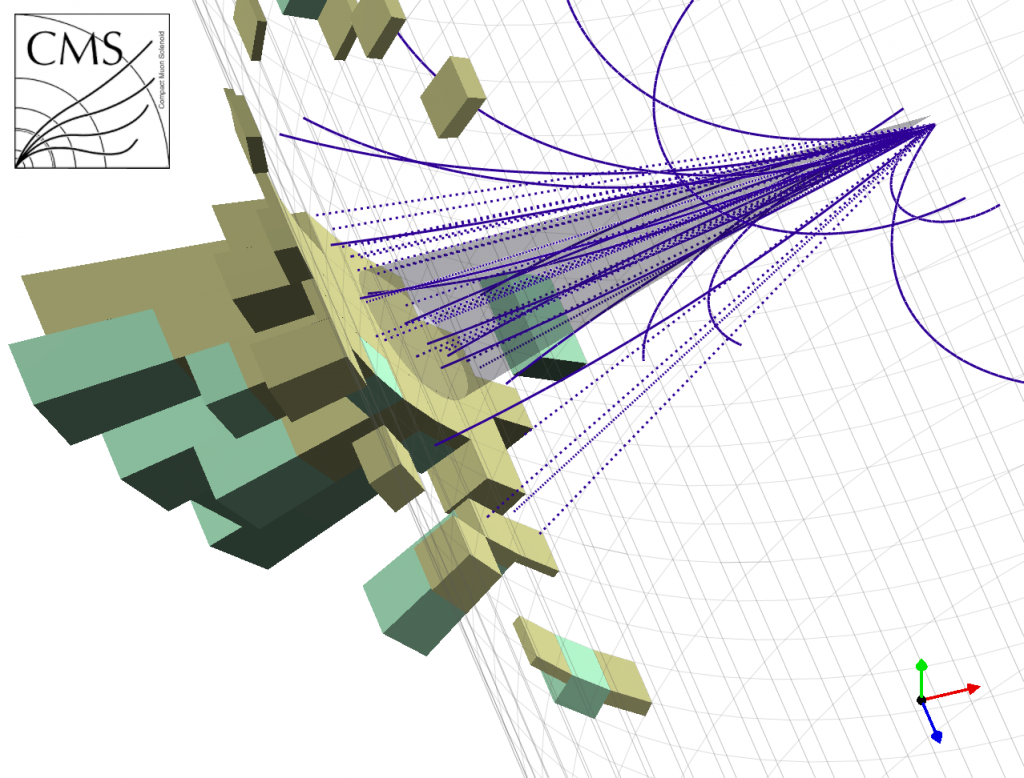
\includegraphics[width=0.45\textwidth]{figures/jetClusteringInCMS.png}
	\caption{A cone of reconstructed particles reconstructed as a jet, with the reconstructed vertex on the right.  
	From the CMS Experiment.}
	\label{fig:jetClustering}
\end{figure}


\section{Trigger and Offline Selection Criteria}
\label{sec:onlineAndOfflineIdSel}
During collisions, in the high-level trigger the electron, muon, and HCAL cluster reconstruction algorithms are used to reconstruct 
electrons and muons.  Then, trigger selection criteria are applied to select events that have two electrons or one muon that is isolated 
from other particles and has a large transverse energy: $\pt > 50$ $\GeV$ for a muon, and $\Et > 33$ $\GeV$ for both electrons.  Offline, 
particles in each event are reconstructed using information from the entire detector, and then additional selection 
criteria are applied to the reconstructed leptons and jets.  Events that met the selection criteria, described in detail in Appendix 
\ref{app_trgOfflId}, had two same flavor leptons and at least two jets with the following characteristics:
\newline

\textbf{Electrons}
\begin{itemize}
	\item The $\Et$ of each electron was equal to the energy of its SC measured in the ECAL.
	\item Each electron had an $\Et > 33$ $\GeV$, and an $|\eta| < 1.44$ or an $|\eta| > 1.57$.
	\item The majority of each electron's energy in the ECAL was measured in a region that was 2 crystals wide in $\eta$.
	\item Each electron was promptly produced, and was not reconstructed near other particles.
	\item The track of each electron was reconstructed from multiple high quality measurements made in the tracker.
\end{itemize}
\newline

\textbf{Muons}
\begin{itemize}
	\item Each muon had an $|\eta| < 2.4$, and at least one muon had a $\pt > 50$ $\GeV$.
	\item Each muon was promptly produced, and was not reconstructed near other charged particles.
	\item Each muon was reconstructed from multiple high quality measurements made in the tracker and the muon detectors.
\end{itemize}
\newline

\textbf{Jets}
\begin{itemize}
	\item Each jet had at least two particles, and at least one was a charged hadron.
	\item More than 0\% of the total energy of each jet came from charged hadrons.
	\item Less than 90\% of the total energy of each jet came from neutral hadrons.
	\item Less than 90\% of the total energy of each jet came from photons.
	\item Less than 99\% of the total energy of each jet came from electrons.
\end{itemize}

Leptons reconstructed in simulated events passed the trigger and offline selection criteria with a different efficiency than leptons 
reconstructed in data events.  This efficiency difference was corrected by multiplying the weight of each selected simulated event by 
0.989 for each electron, by a $\pt$,$\eta$-dependent value between 0.99 and 1.0 for each muon, and by an additional $\pt$,$\eta$-
dependent value between 0.95 and 1.04 for the muon that passed the trigger selection criteria.


\section{\WR Kinematics and Offline Kinematic Selection Criteria}
\label{sec:signalAndBkgnds}
The trigger and offline selection criteria described previously were used to select events where two leptons and jets are identified.  
These selection criteria were also used in other searches for heavy particles that decay to leptons and jets \cite{exoLeptJetResults}, 
and were not specifically optimized for this analysis.

Having selected events for this search, the leptons and jets were required to pass additional selection criteria that were motivated by 
the kinematics of the \WR progeny.  The heavy \WR decays through a lighter \nul to two leptons and two jets according to the following 
decay chain:

\begin{equation}
	\WR \rightarrow \nul \plus \ell_{1} ; \quad \nul \rightarrow \ell_{2} jj
\end{equation}
%\begin{tikzpicture}[grow=right]
%	\node (Wr) at (0,0) {$\WR \thickspace \rightarrow \thickspace \nul + \ell$};
%	\node (Ar) at (0.75,-0.4) {$\searrow$};
%	\node (Nl) at (1.25,-0.75) {$\ell jj$};
%\end{tikzpicture} $\newline$
Since the \WR and \nul are assumed to couple to leptons and quarks with the same strengths as the $W$, the \WR and \nul decay promptly 
to leptons and quarks that hadronize into jets.  The kinematics of these particles are governed by the \WR mass and the ratio $\mnul/\mWR$.

Since the \WR mass is expected to be several $\TeV$ the \WR has low net momentum, and its progeny \nul and $\ell_{1}$ are emitted 
isotropically in the lab frame.  As a result, the $\ell_{1}$ and the \nul progeny are emitted in the region $|\eta| < 2.4$, as shown in 
Figure \ref{fig:wrLeptJetEtas}.  Therefore, both reconstructed leptons and jets were required to have an $|\eta| < 2.4$.

\begin{figure}
	\centering
	\begin{subfigure}[t]{2.4in}
		\centering
		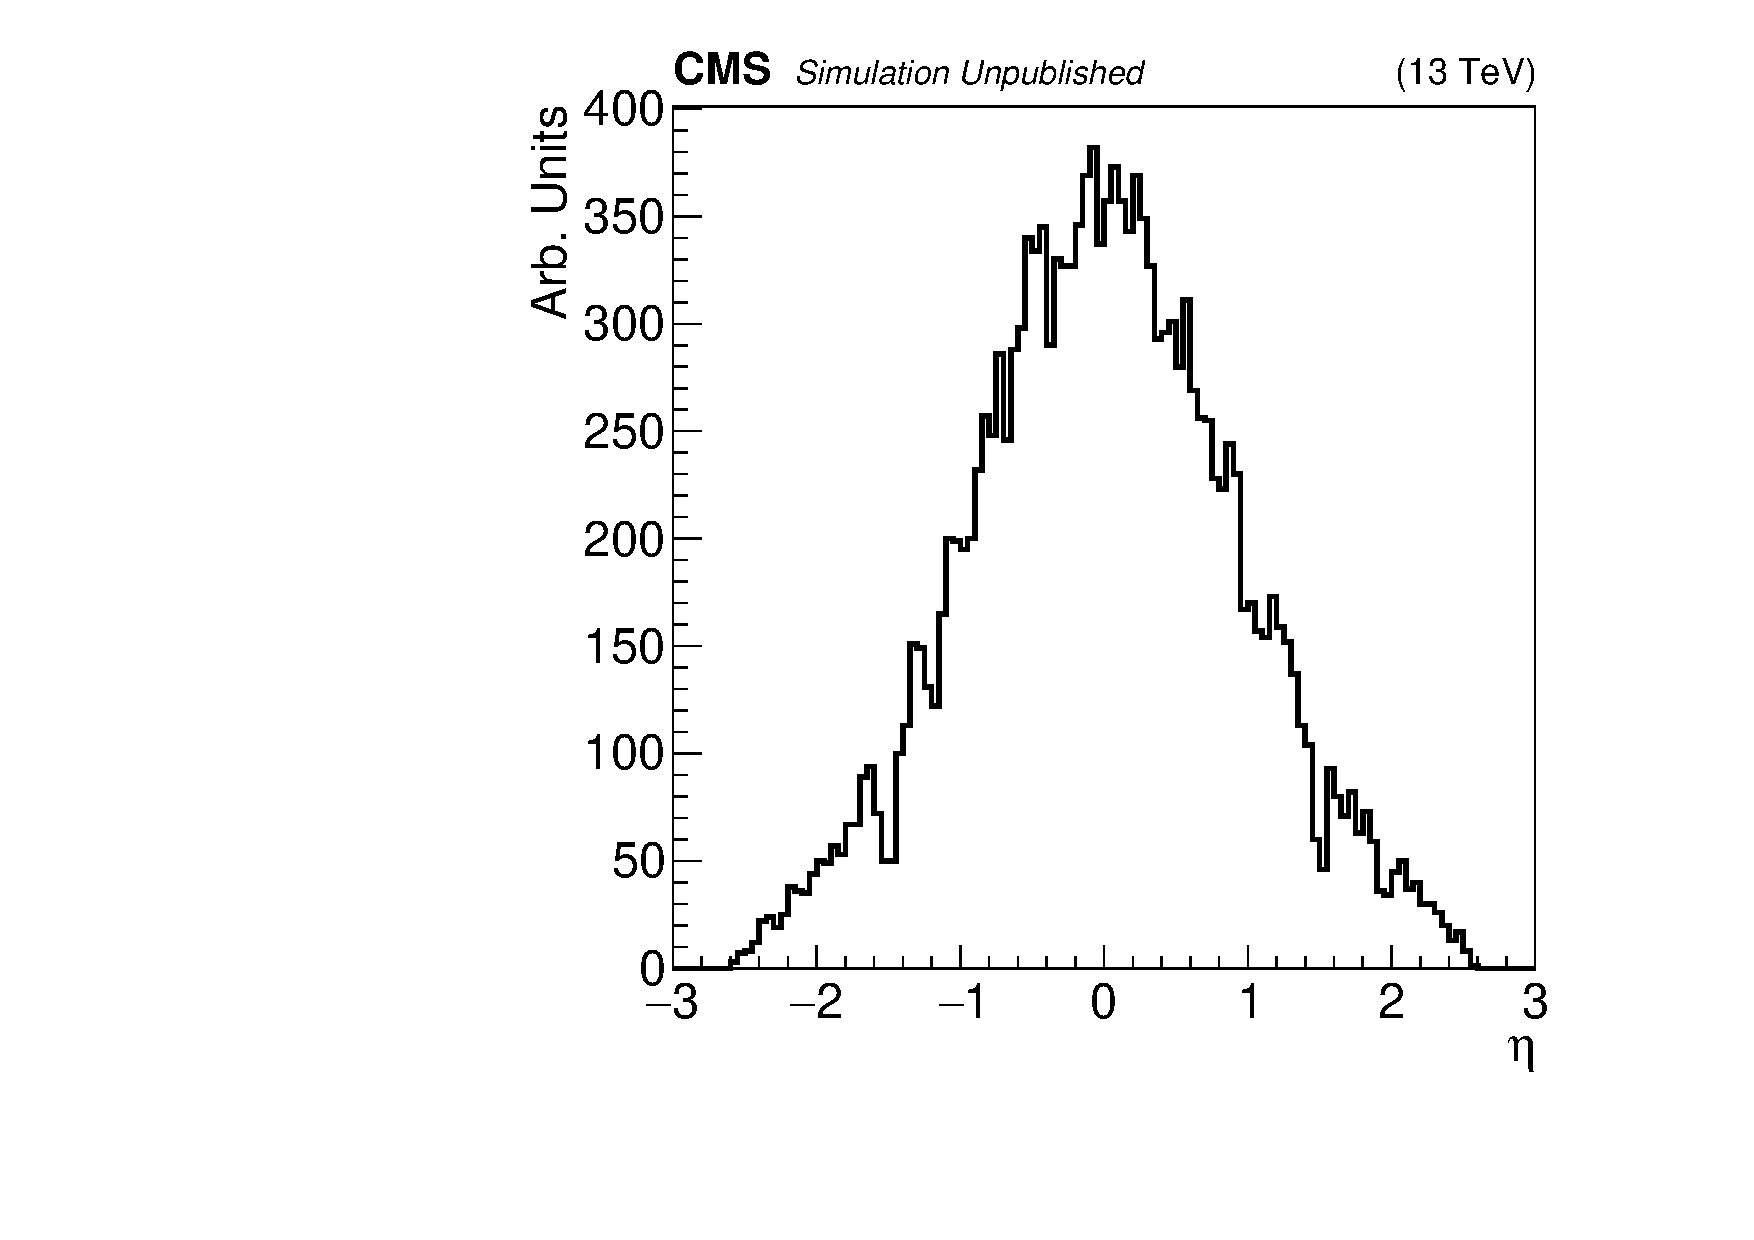
\includegraphics[width=2.4in]{figures/etaMatchedRecoEleFromWr_mwr2200_mnu1100.pdf}
		\caption{$\ell$ from $\WR \rightarrow \ell\nul$}\label{fig:wrLeptJetEtasa}
	\end{subfigure}
	\thickspace
	\begin{subfigure}[t]{2.4in}
		\centering
		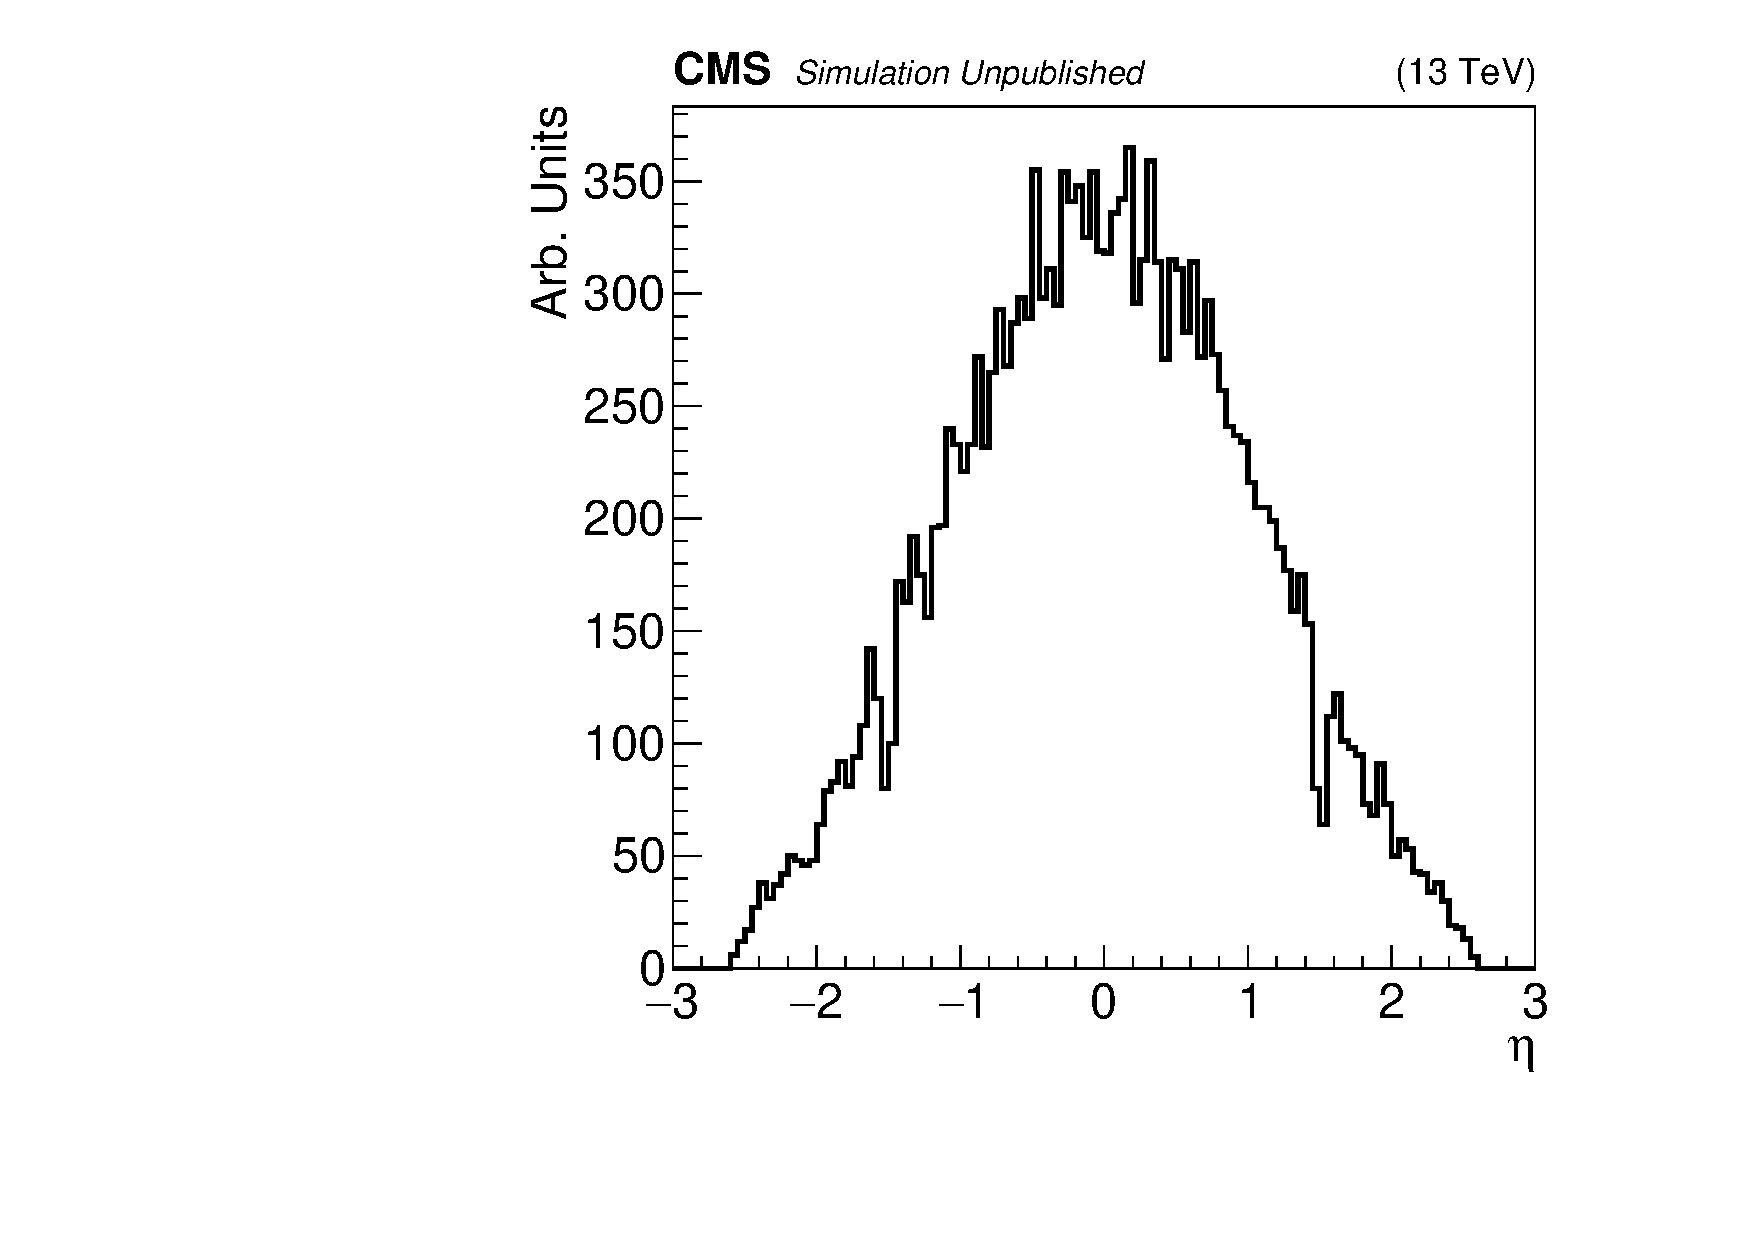
\includegraphics[width=2.4in]{figures/etaMatchedRecoEleFromNu_mwr2200_mnu1100.pdf}
		\caption{$\ell$ from $\nul \rightarrow \ell jj$}\label{fig:wrLeptJetEtasb}
	\end{subfigure}
	\newline
	\newline
	\newline
	\newline
	\begin{subfigure}[t]{2.4in}
		\centering
		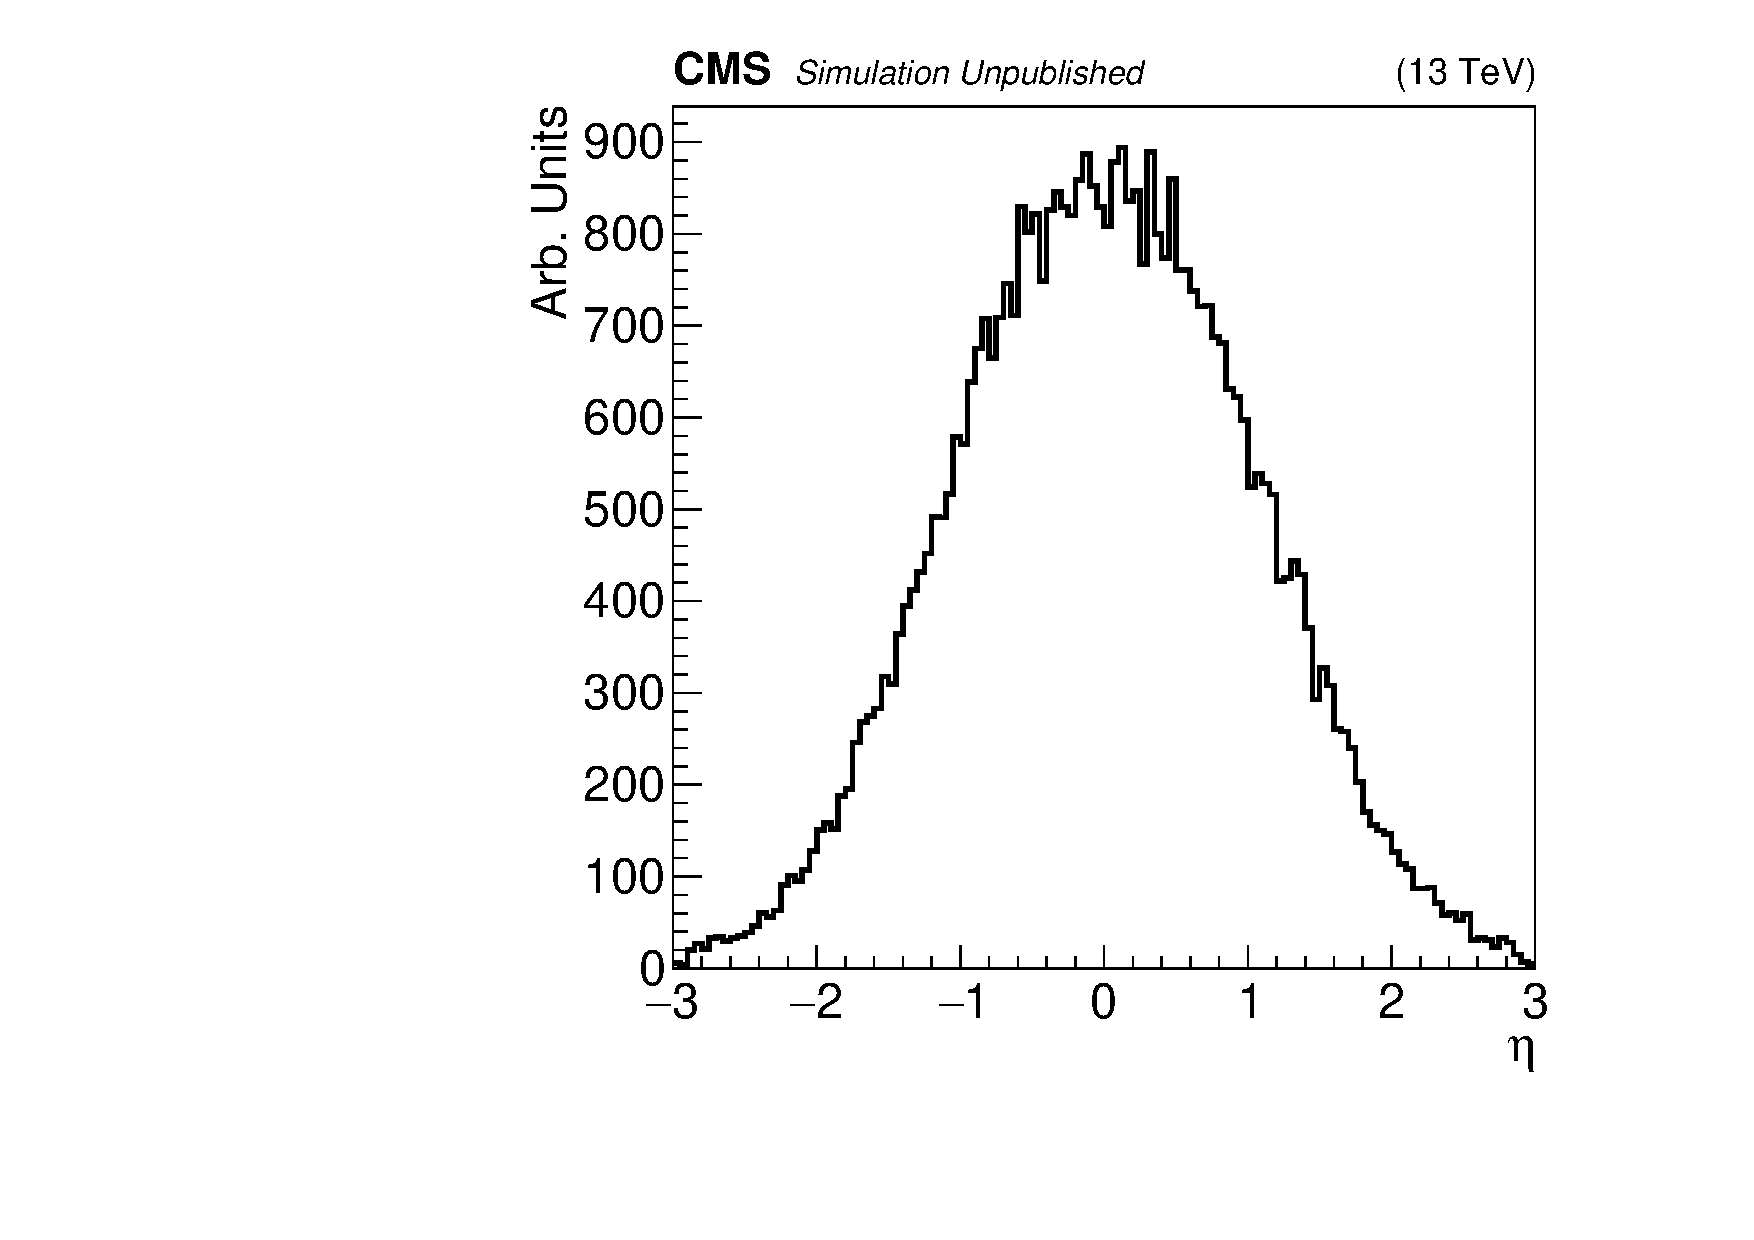
\includegraphics[width=2.4in]{figures/etaMatchedRecoJetOne_mwr2200_mnu1100.pdf}
		\caption{jet from $\nul \rightarrow \ell jj$}\label{fig:wrLeptJetEtasc}
	\end{subfigure}
	\thickspace
	\begin{subfigure}[t]{2.4in}
		\centering
		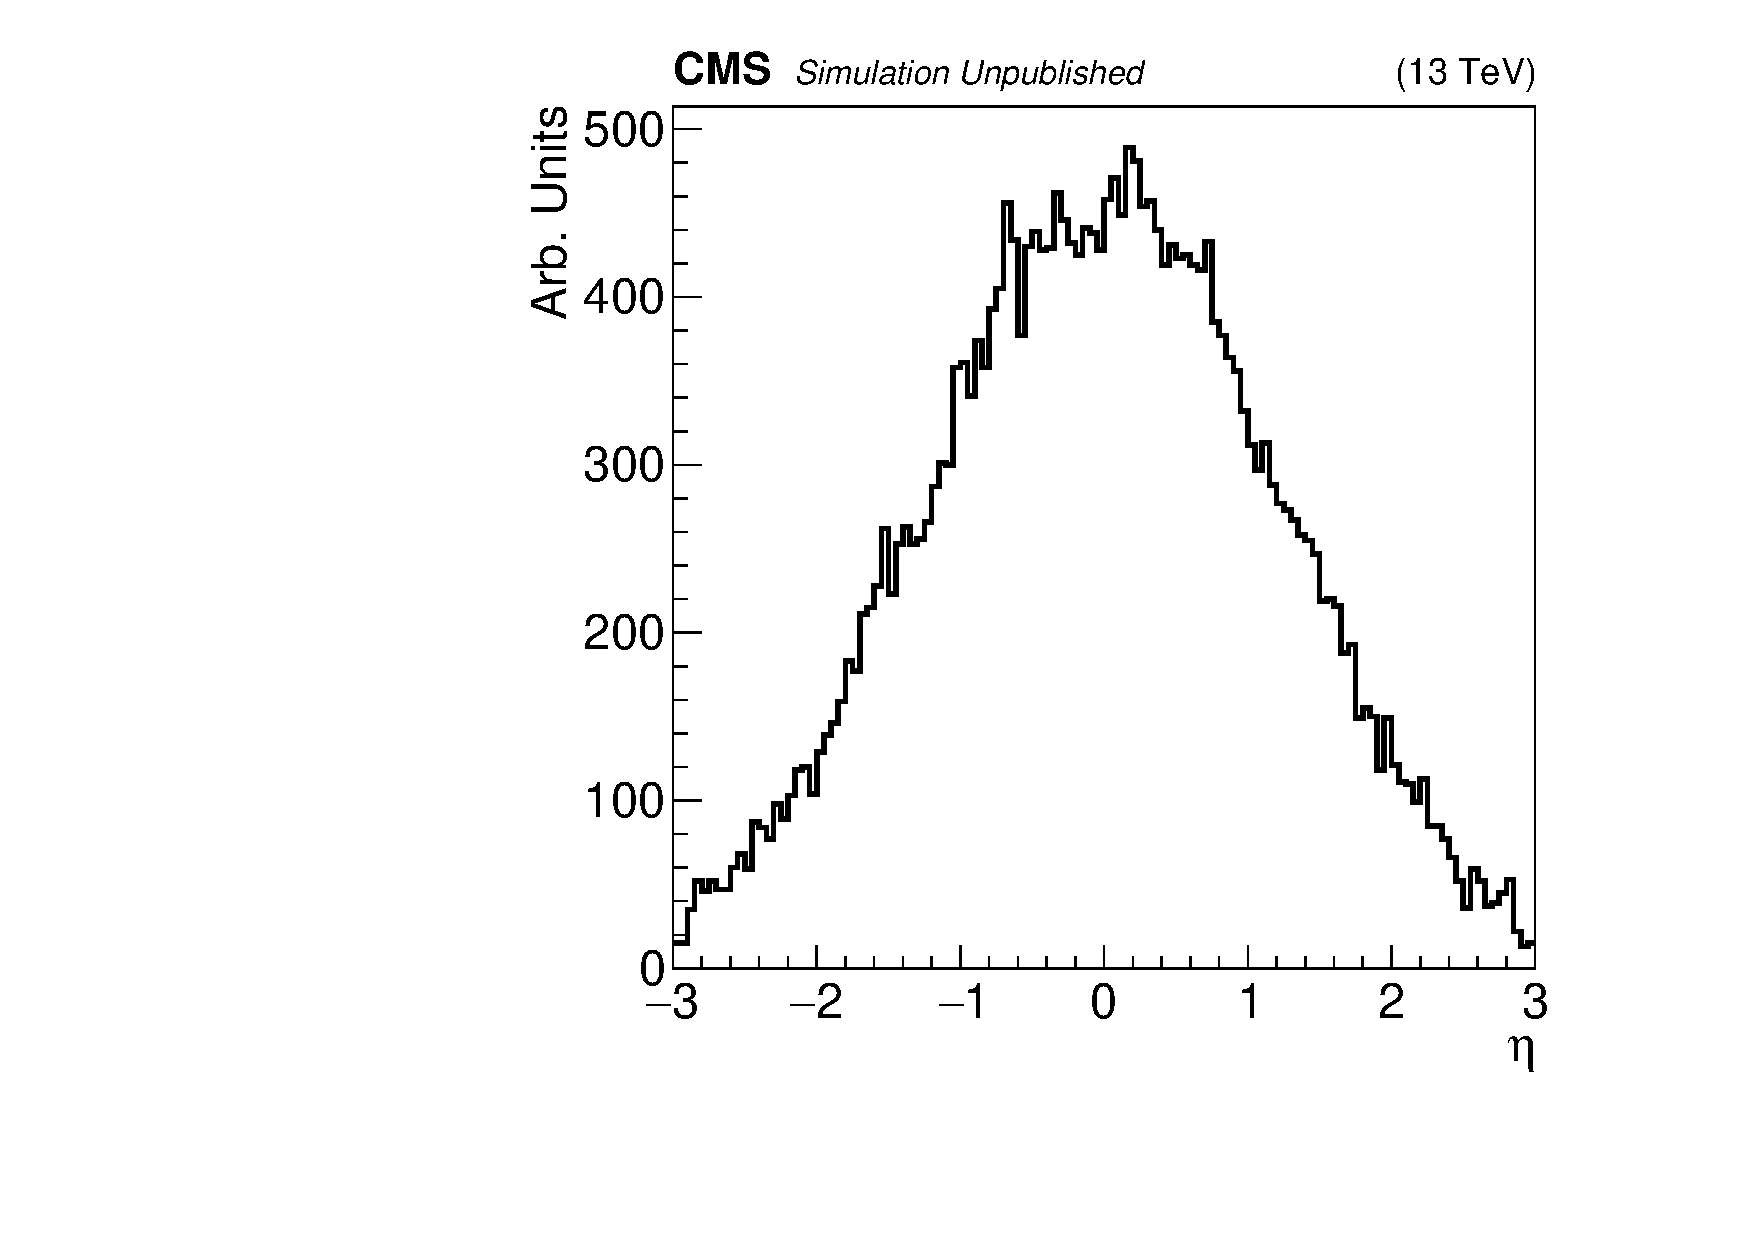
\includegraphics[width=2.4in]{figures/etaMatchedRecoJetTwo_mwr2200_mnu1100.pdf}
		\caption{jet from $\nul \rightarrow \ell jj$}\label{fig:wrLeptJetEtasd}
	\end{subfigure}
	\caption{The $\eta$ distributions of leptons and jets reconstructed in $\WR \rightarrow \ell\ell jj$ events with $\mWR = 2.2$ $\TeV$ 
		and $\mnul = \frac{1}{2}\mWR$.}\label{fig:wrLeptJetEtas}
\end{figure}
\clearpage

In the decay $\nul \rightarrow \ell_{2} q_{1}q_{2}$, the ratio $\mnul/\mWR$ affects the $\Delta R(\ell,q)$ separation between the lepton 
and the two quarks.  As $\mnul/\mWR$ decreases from 1 to 0 the \nul momentum magnitude increases, as shown in Figure 
\ref{fig:hvyNuMomentumVarMNu}.  As the \nul momentum increases the $\ell_{2}$ and both quarks produced in the \nul decay are boosted 
along the \nul direction of momentum in the lab frame.  As $\mnul/\mWR$ decreases this boost increases, causing the $\Delta R(\ell,q)$ 
separation between the $\ell_{2}$ and both quarks to decrease, as shown in Figure \ref{fig:wrDrLeptQrkVarMNu}.  Since the lepton 
reconstructed from $\ell_{2}$ can also be reconstructed as part of a jet, as $\Delta R(\ell,q)$ decreases the probability increases that 
a jet is reconstructed from $\ell_{2}$ and either $q_{1}$ or $q_{2}$, and passes the selection criteria.  In addition, there is a low 
probability, independent of $\mnul/\mWR$, that the lepton produced in the decay $\WR \rightarrow \ell_{1} \nul$ is emitted in the vicinity 
of $q_{1}$ or $q_{2}$, and $\ell_{1}$ and one quark are reconstructed as a jet that passes the selection criteria.  To avoid selecting 
jets that are reconstructed from combinations of $\ell_{1}$ or $\ell_{2}$ and $q_{1}$ or $q_{2}$, each jet was required to be separated 
from each selected lepton by $\Delta R > 0.4$.

\begin{figure}[h]
	\centering
	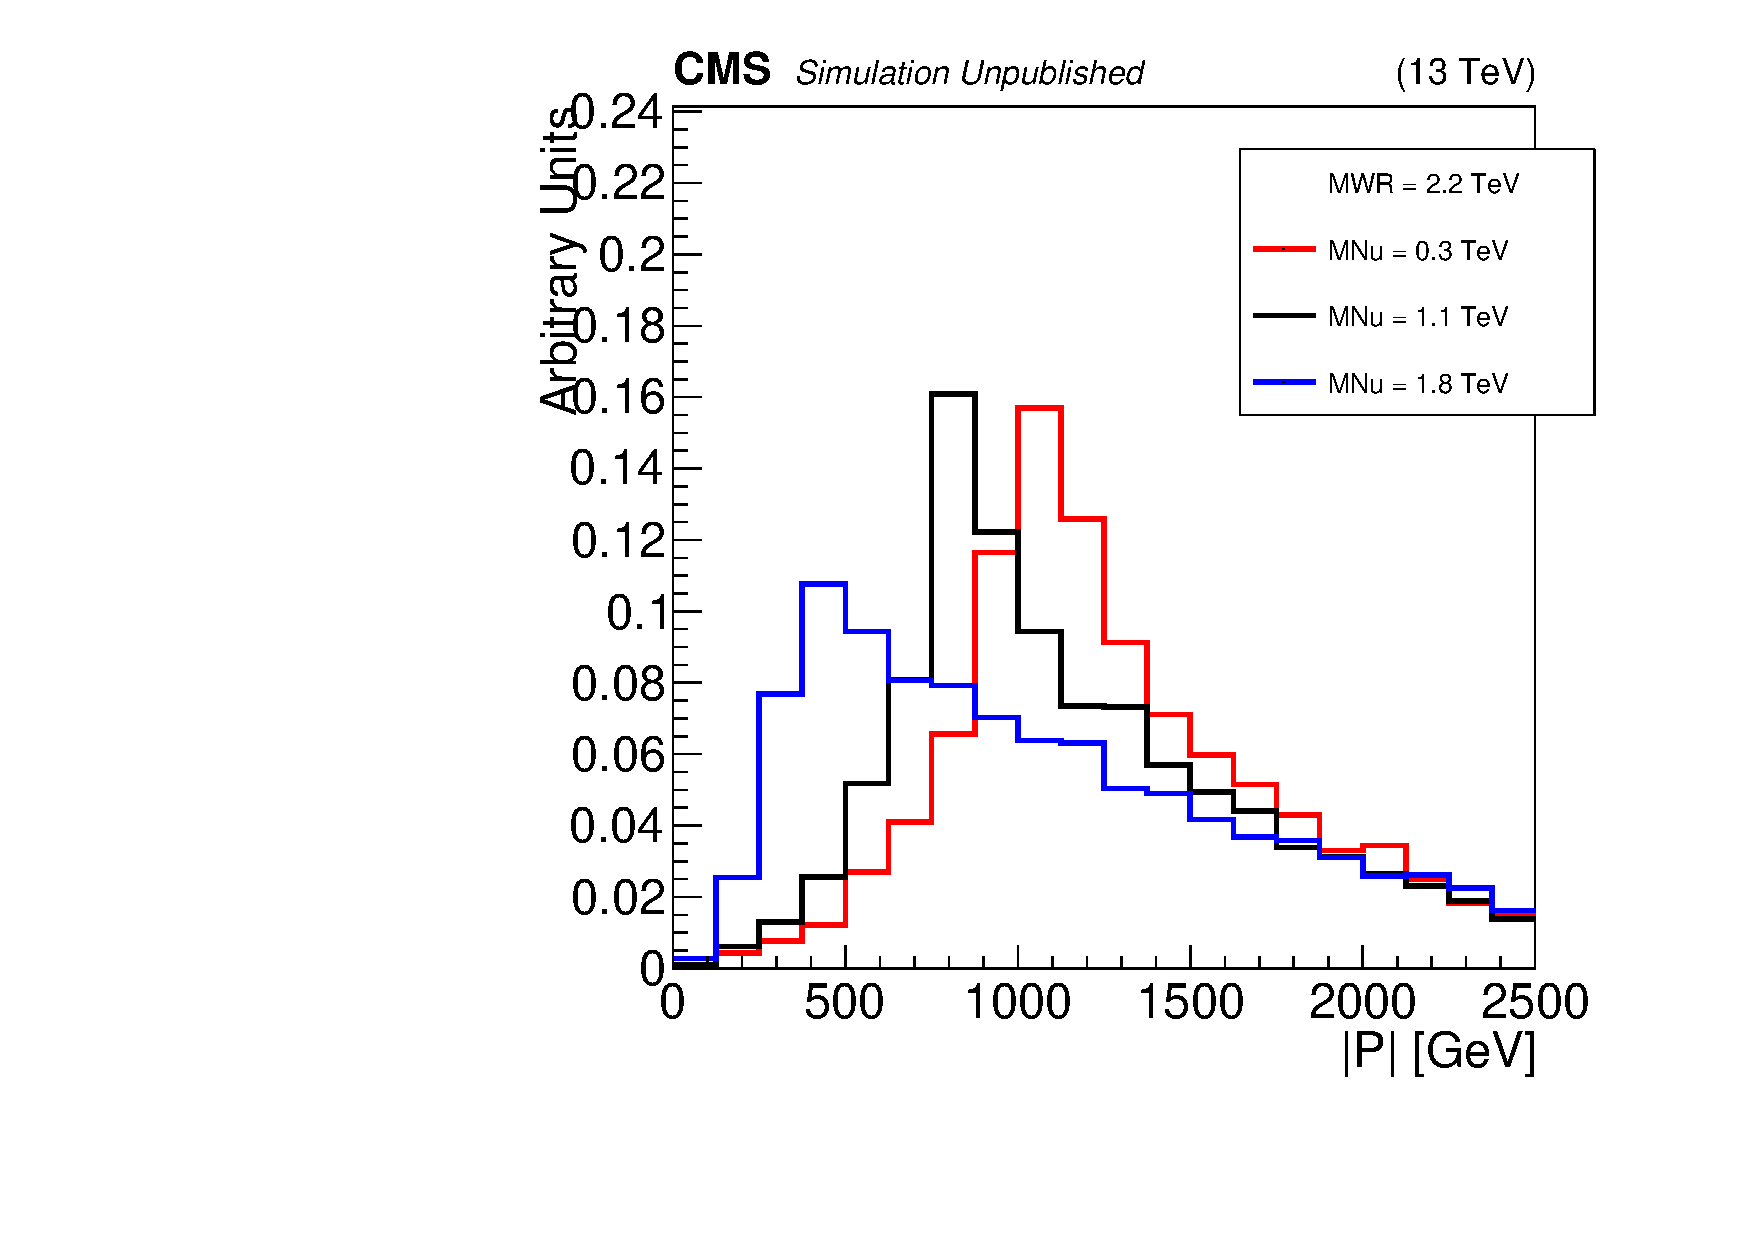
\includegraphics[width=0.5\textwidth]{figures/genNuMomMag_MWR_2200_several_MNu_private.pdf}
	\caption{The $|p|$ distribution of the \nul produced in $\WR \rightarrow \ell\nul$ events with $\mWR = 2.2$ $\TeV$ and different \mnul.}
	\label{fig:hvyNuMomentumVarMNu}
\end{figure}

\begin{figure}
	\centering
	\begin{subfigure}[t]{2.4in}
		\centering
		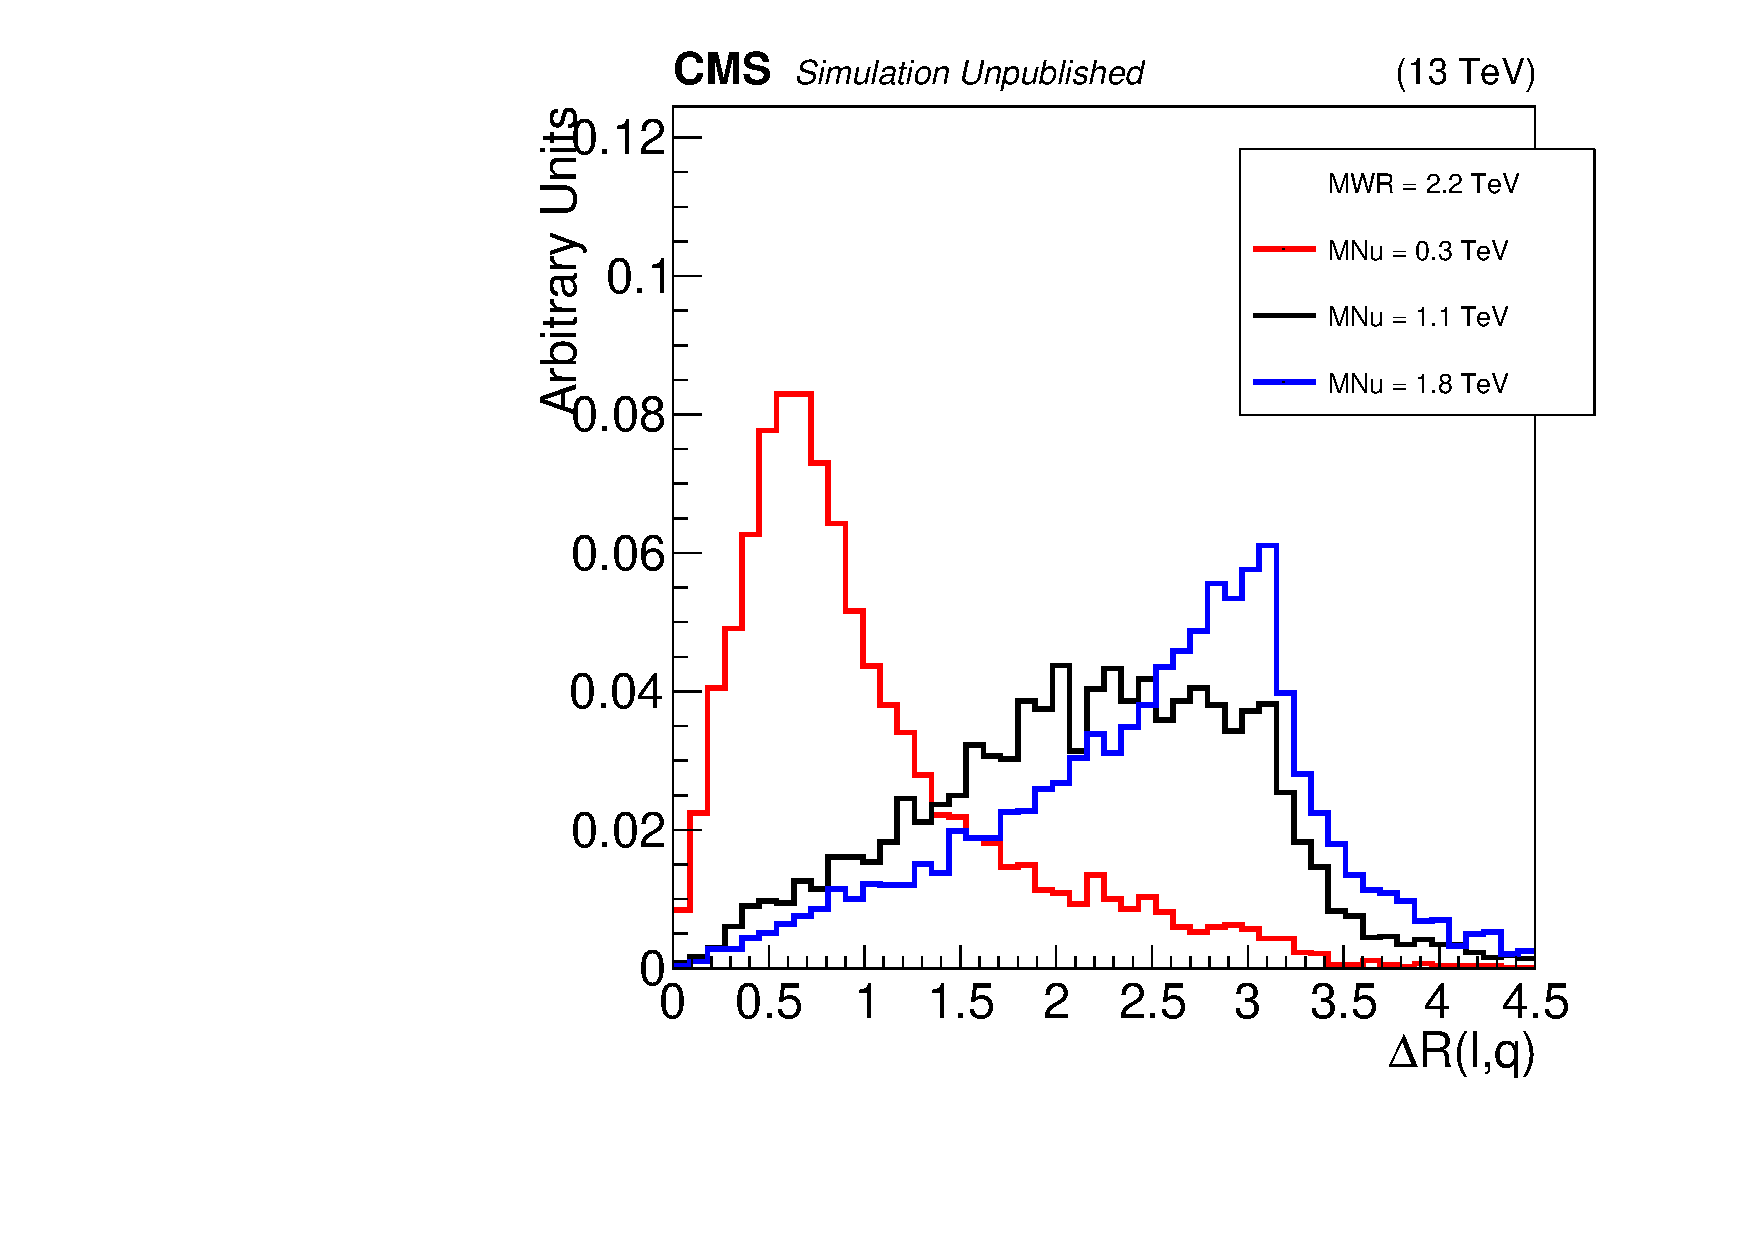
\includegraphics[width=2.4in]{figures/dRgenLeptonFromScdHvyPtclGenQuarkOneFromScdHvyPtcl_MWR_2200_several_MNu_private.pdf}
		%\caption{ }\label{fig:wrDrLeptQrkVarMNua}
	\end{subfigure}
	\thickspace
	\begin{subfigure}[t]{2.4in}
		\centering
		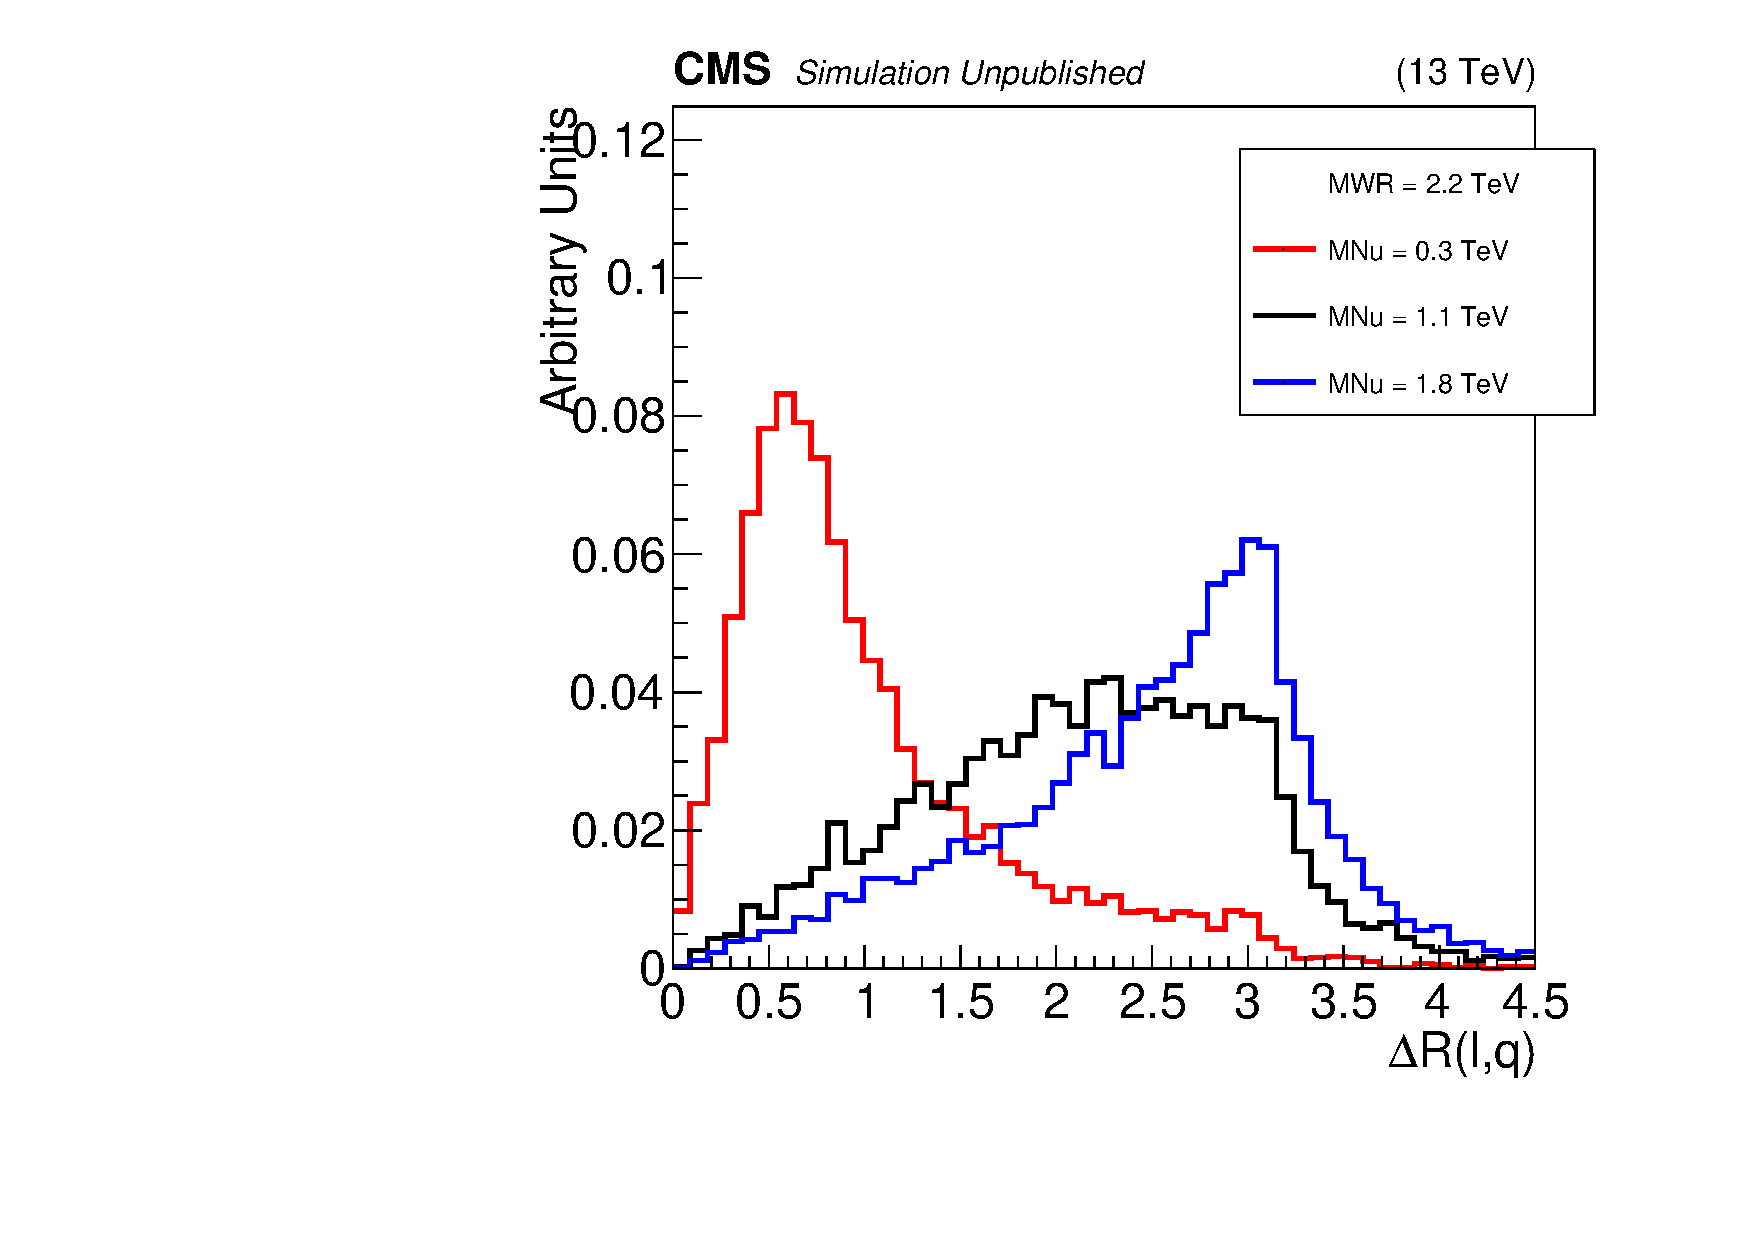
\includegraphics[width=2.4in]{figures/dRgenLeptonFromScdHvyPtclGenQuarkTwoFromScdHvyPtcl_MWR_2200_several_MNu_private.pdf}
		%\caption{ }\label{fig:wrDrLeptQrkVarMNub}
	\end{subfigure}
	\caption{The $\Delta R(\ell,q)$ separation distributions between the $\ell$ and both quarks produced in $\nul \rightarrow \ell qq$ 
		in $\WR \rightarrow \ell\ell qq$ events with $\mWR = 2.2$ $\TeV$ and different \mnul.}\label{fig:wrDrLeptQrkVarMNu}
\end{figure}
\clearpage

The leptons and jets produced in the \WR decay have $\pt$ that are affected by the \WR mass and the ratio $\mnul/\mWR$.  The \WR mass 
represents the total momentum that is distributed amongst the leptons and jets, so the lepton and jet $\pt$ grow with the \WR mass.  
For $\mWR = 2.2$ $\TeV$ and $\mnul = 1.1$ $\TeV$, the average $\pt$ of reconstructed leptons and jets is above 60 $\GeV$, as shown 
in Figure \ref{fig:wrLeptJetPts}.  As $\mnul/\mWR$ increases to 1 the $\pt$ of \nul progeny increase, 
while the $\pt$ of the other lepton decreases, as shown in Figure \ref{fig:wrLeptQrkPtsVarMNu}.  Similarly, as $\mnul/\mWR$ decreases 
to 0 the $\pt$ of both jets decrease, and the $\pt$ of one lepton increases while the $\pt$ of the other lepton decreases.

\begin{figure}
	\centering
	\begin{subfigure}[t]{2.4in}
		\centering
		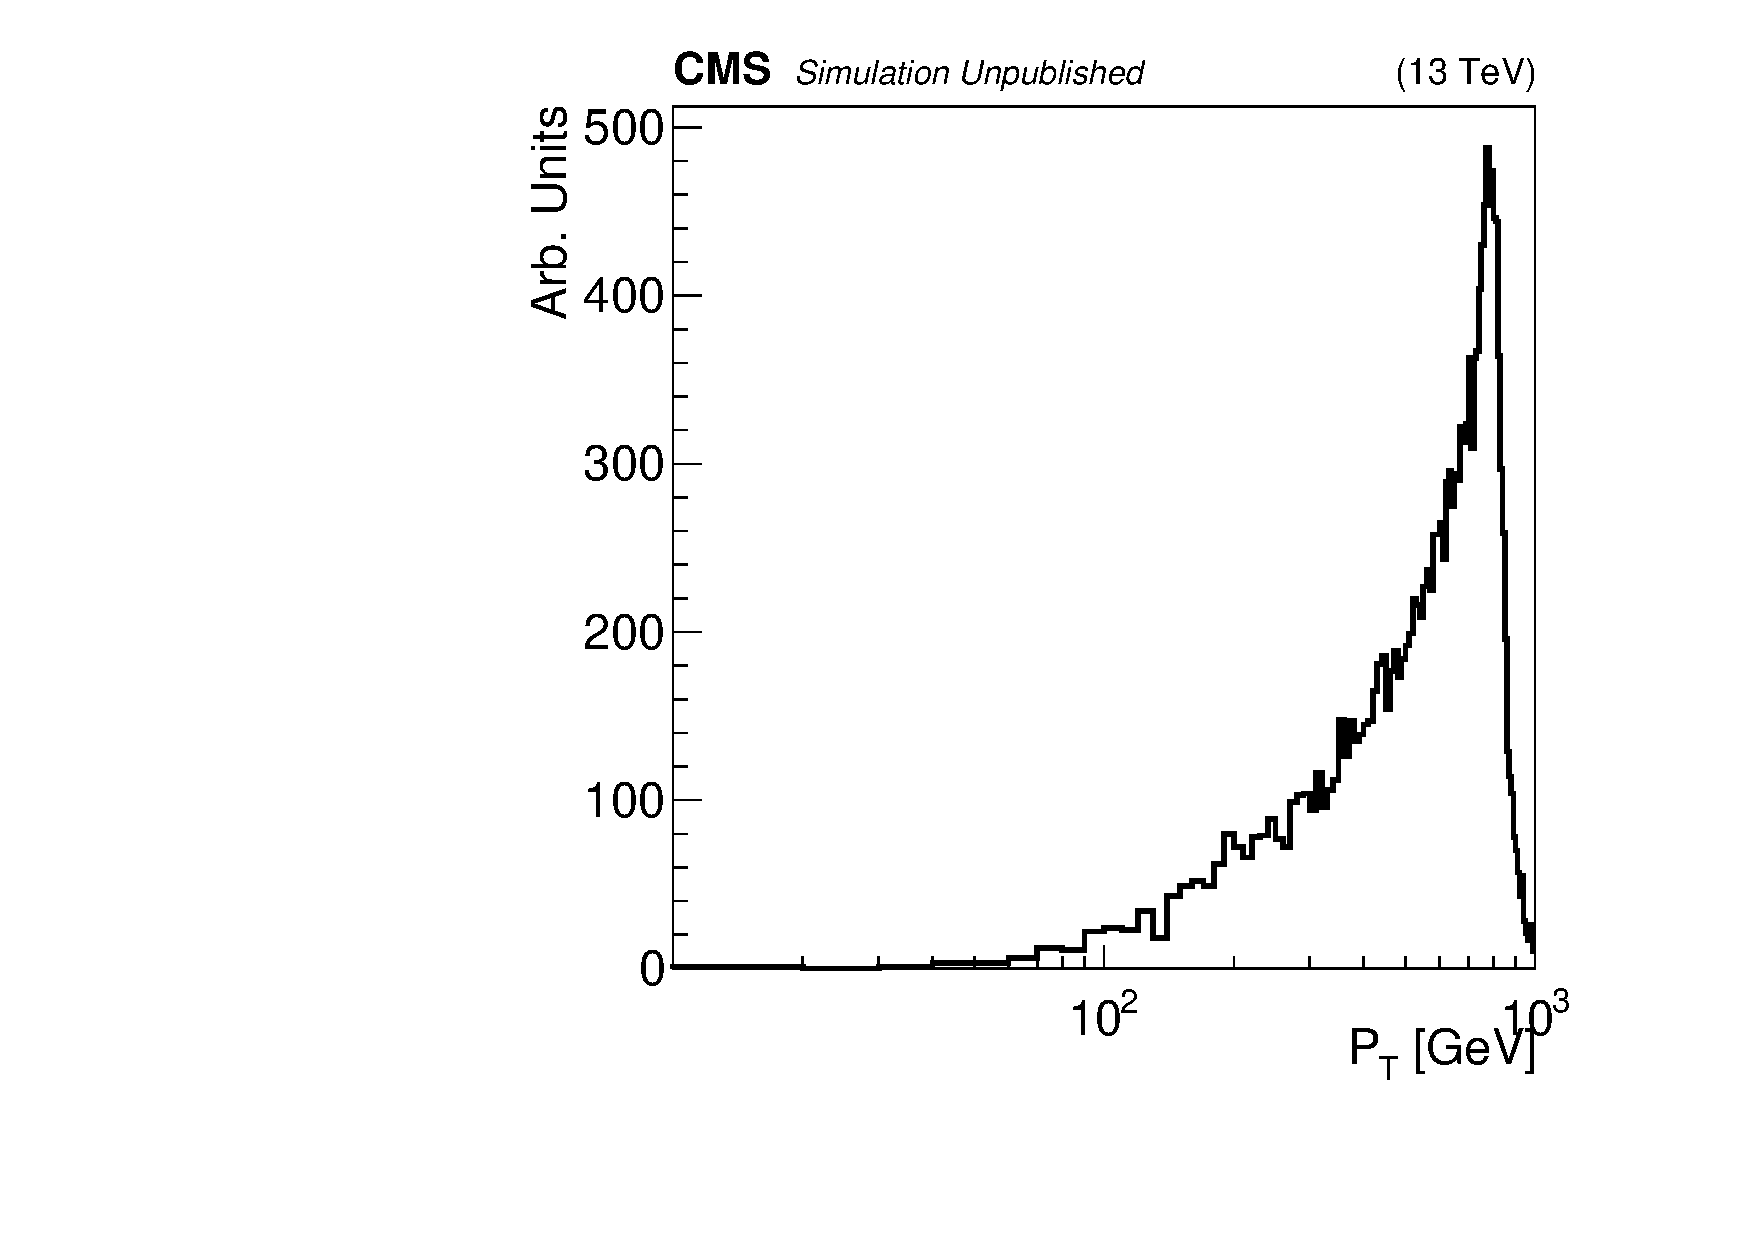
\includegraphics[width=2.4in]{figures/ptMatchedRecoEleFromWr_mwr2200_mnu1100.pdf}
		\caption{$\ell$ from $\WR \rightarrow \ell\nul$}\label{fig:wrLeptJetPtsa}
	\end{subfigure}
	\thickspace
	\begin{subfigure}[t]{2.4in}
		\centering
		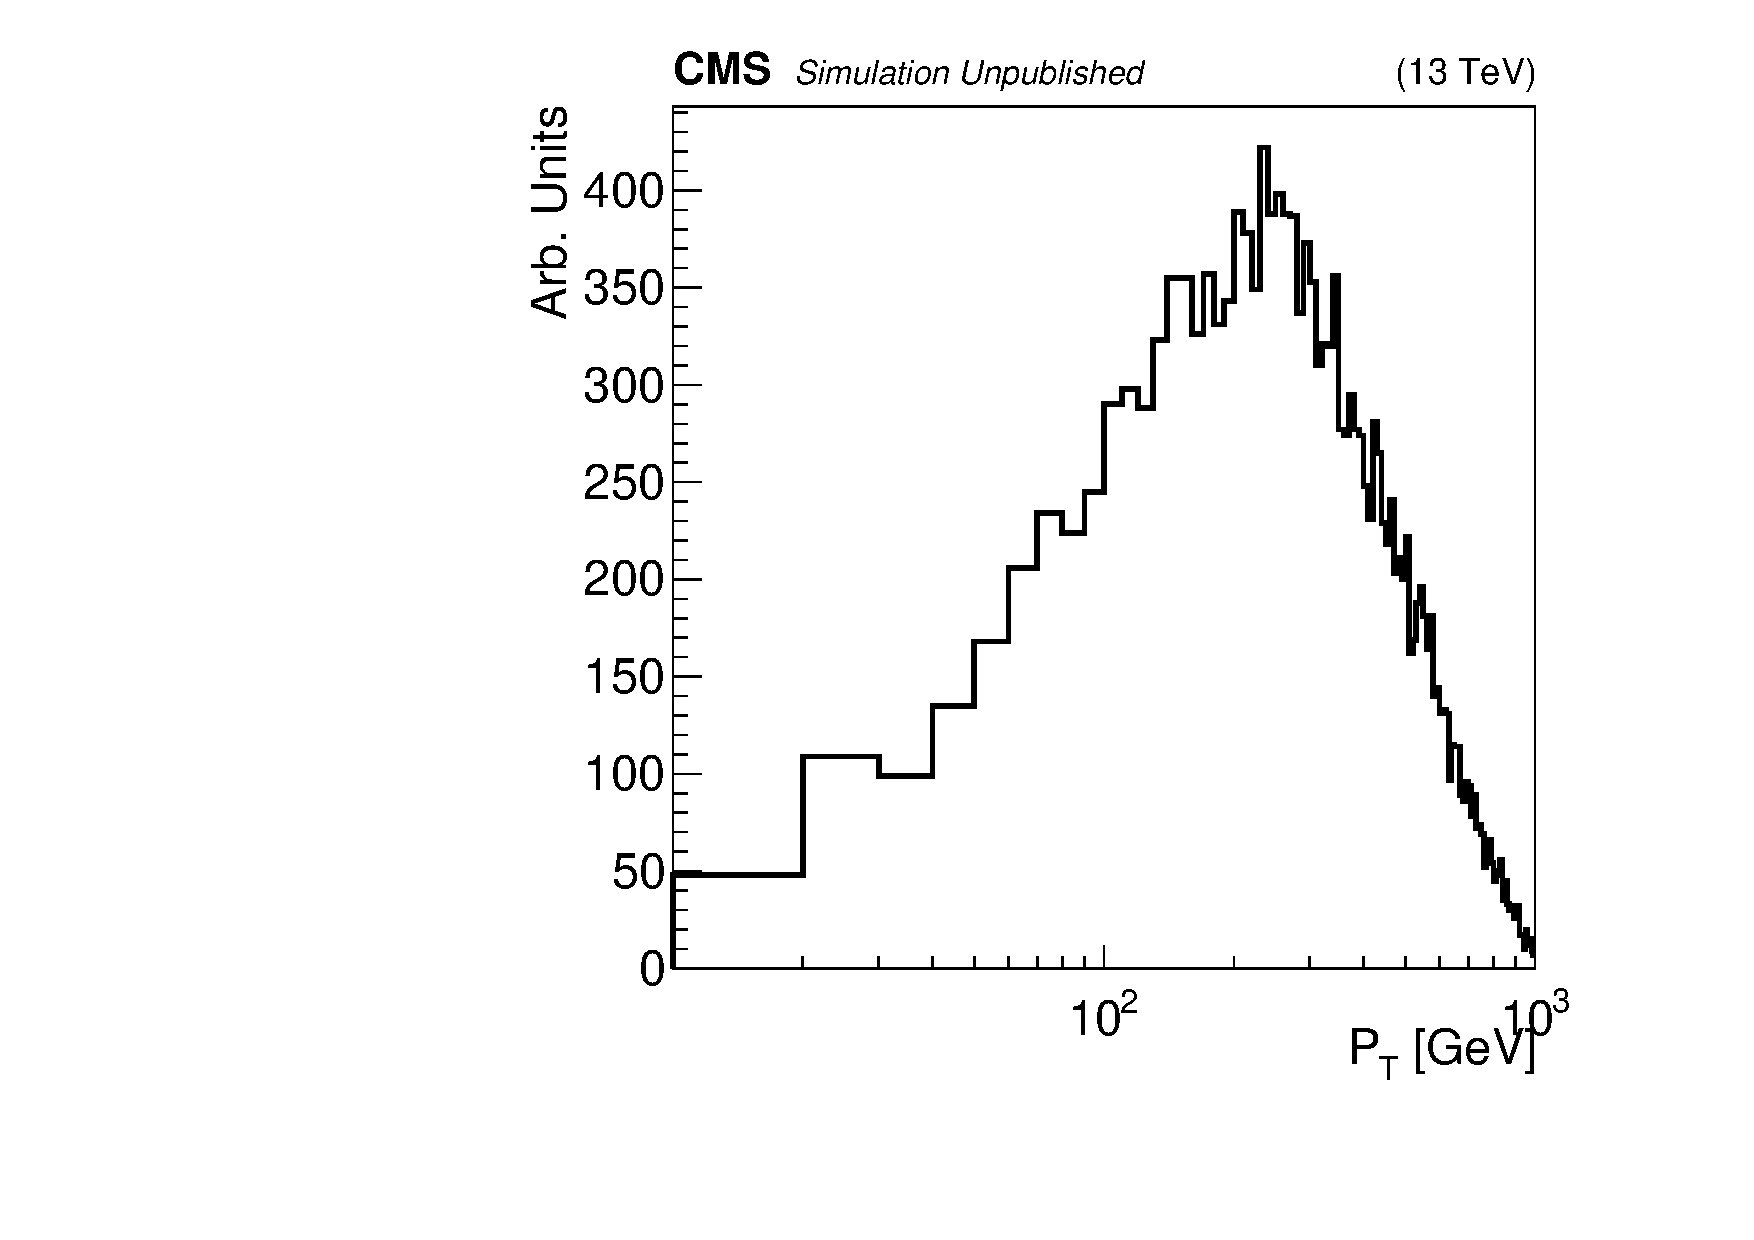
\includegraphics[width=2.4in]{figures/ptMatchedRecoEleFromNu_mwr2200_mnu1100.pdf}
		\caption{$\ell$ from $\nul \rightarrow \ell jj$}\label{fig:wrLeptJetPtsb}
	\end{subfigure}
	\newline
	\newline
	\newline
	\newline
	\begin{subfigure}[t]{2.4in}
		\centering
		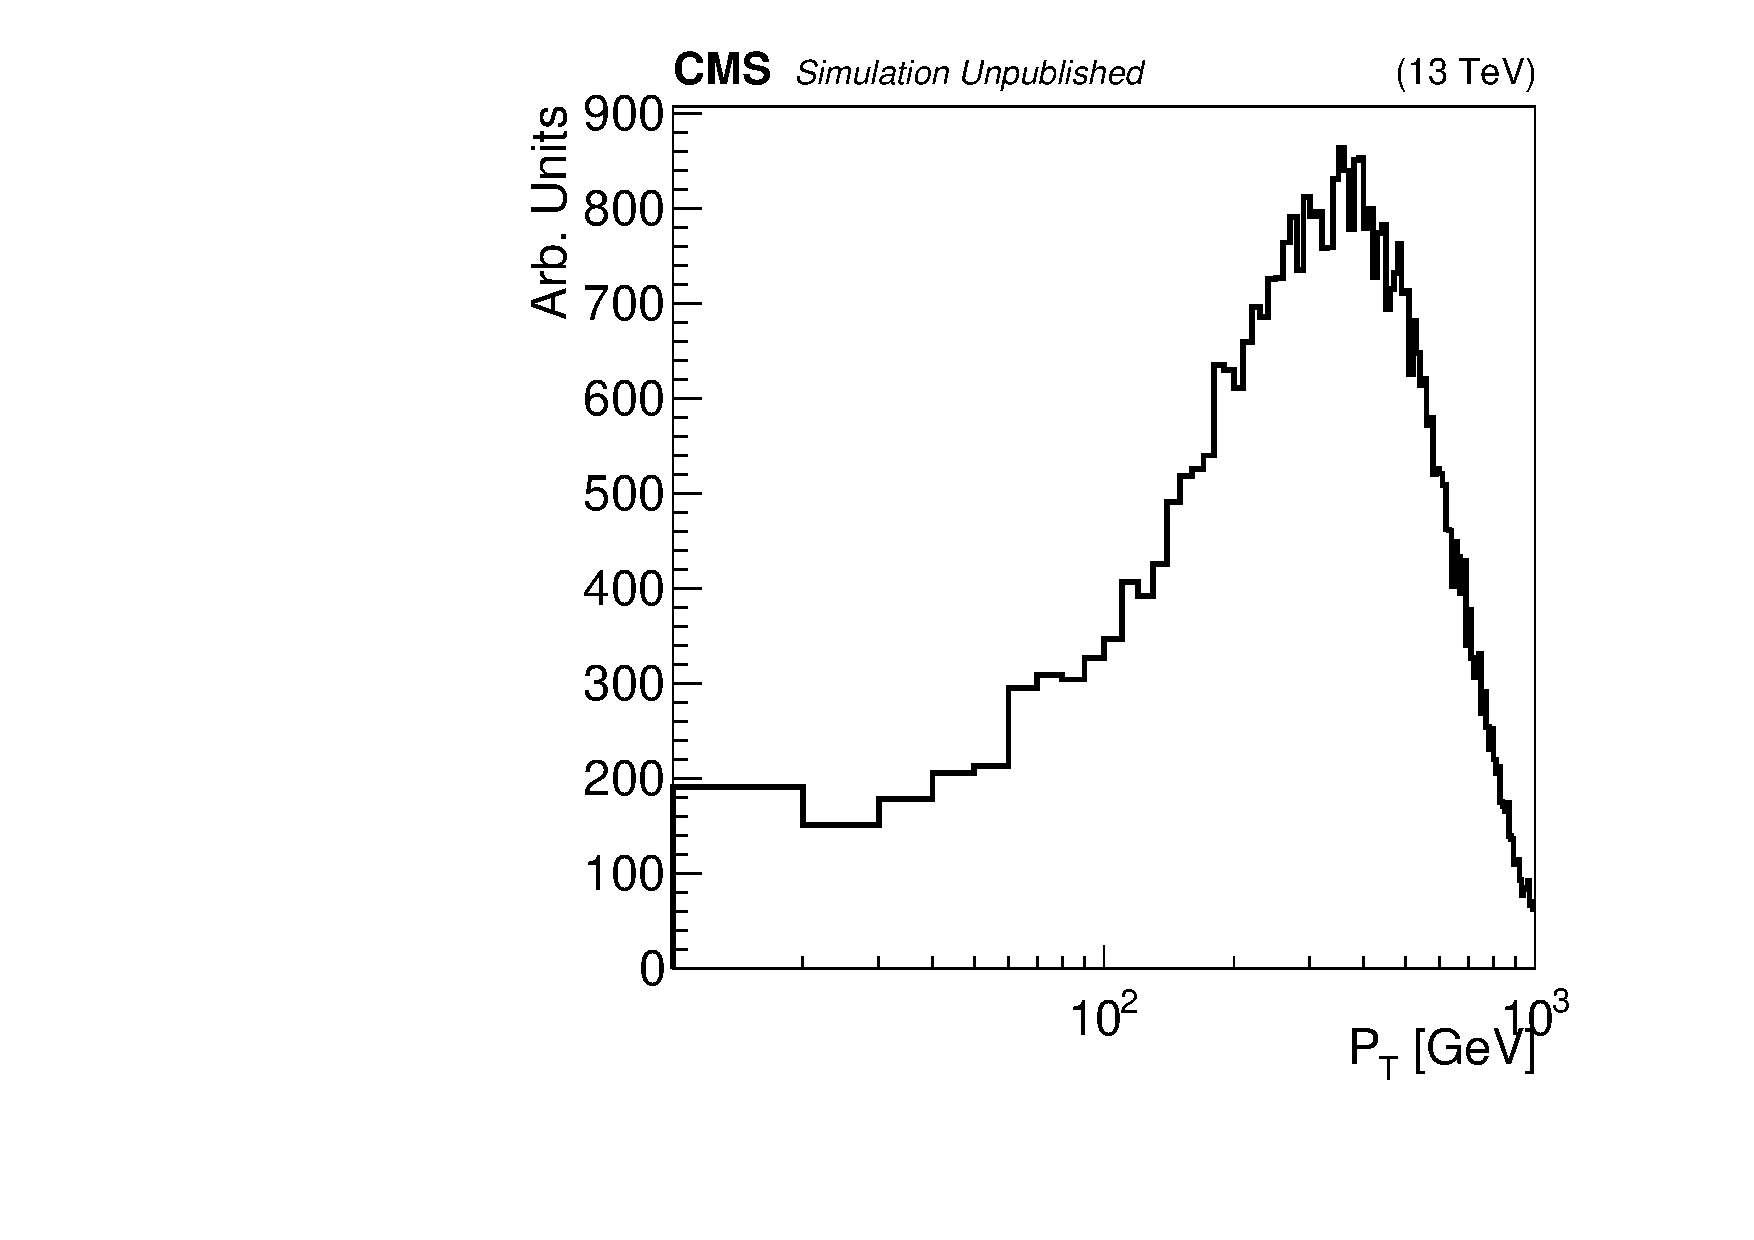
\includegraphics[width=2.4in]{figures/ptMatchedRecoJetOne_mwr2200_mnu1100.pdf}
		\caption{jet from $\nul \rightarrow \ell jj$}\label{fig:wrLeptJetPtsc}
	\end{subfigure}
	\thickspace
	\begin{subfigure}[t]{2.4in}
		\centering
		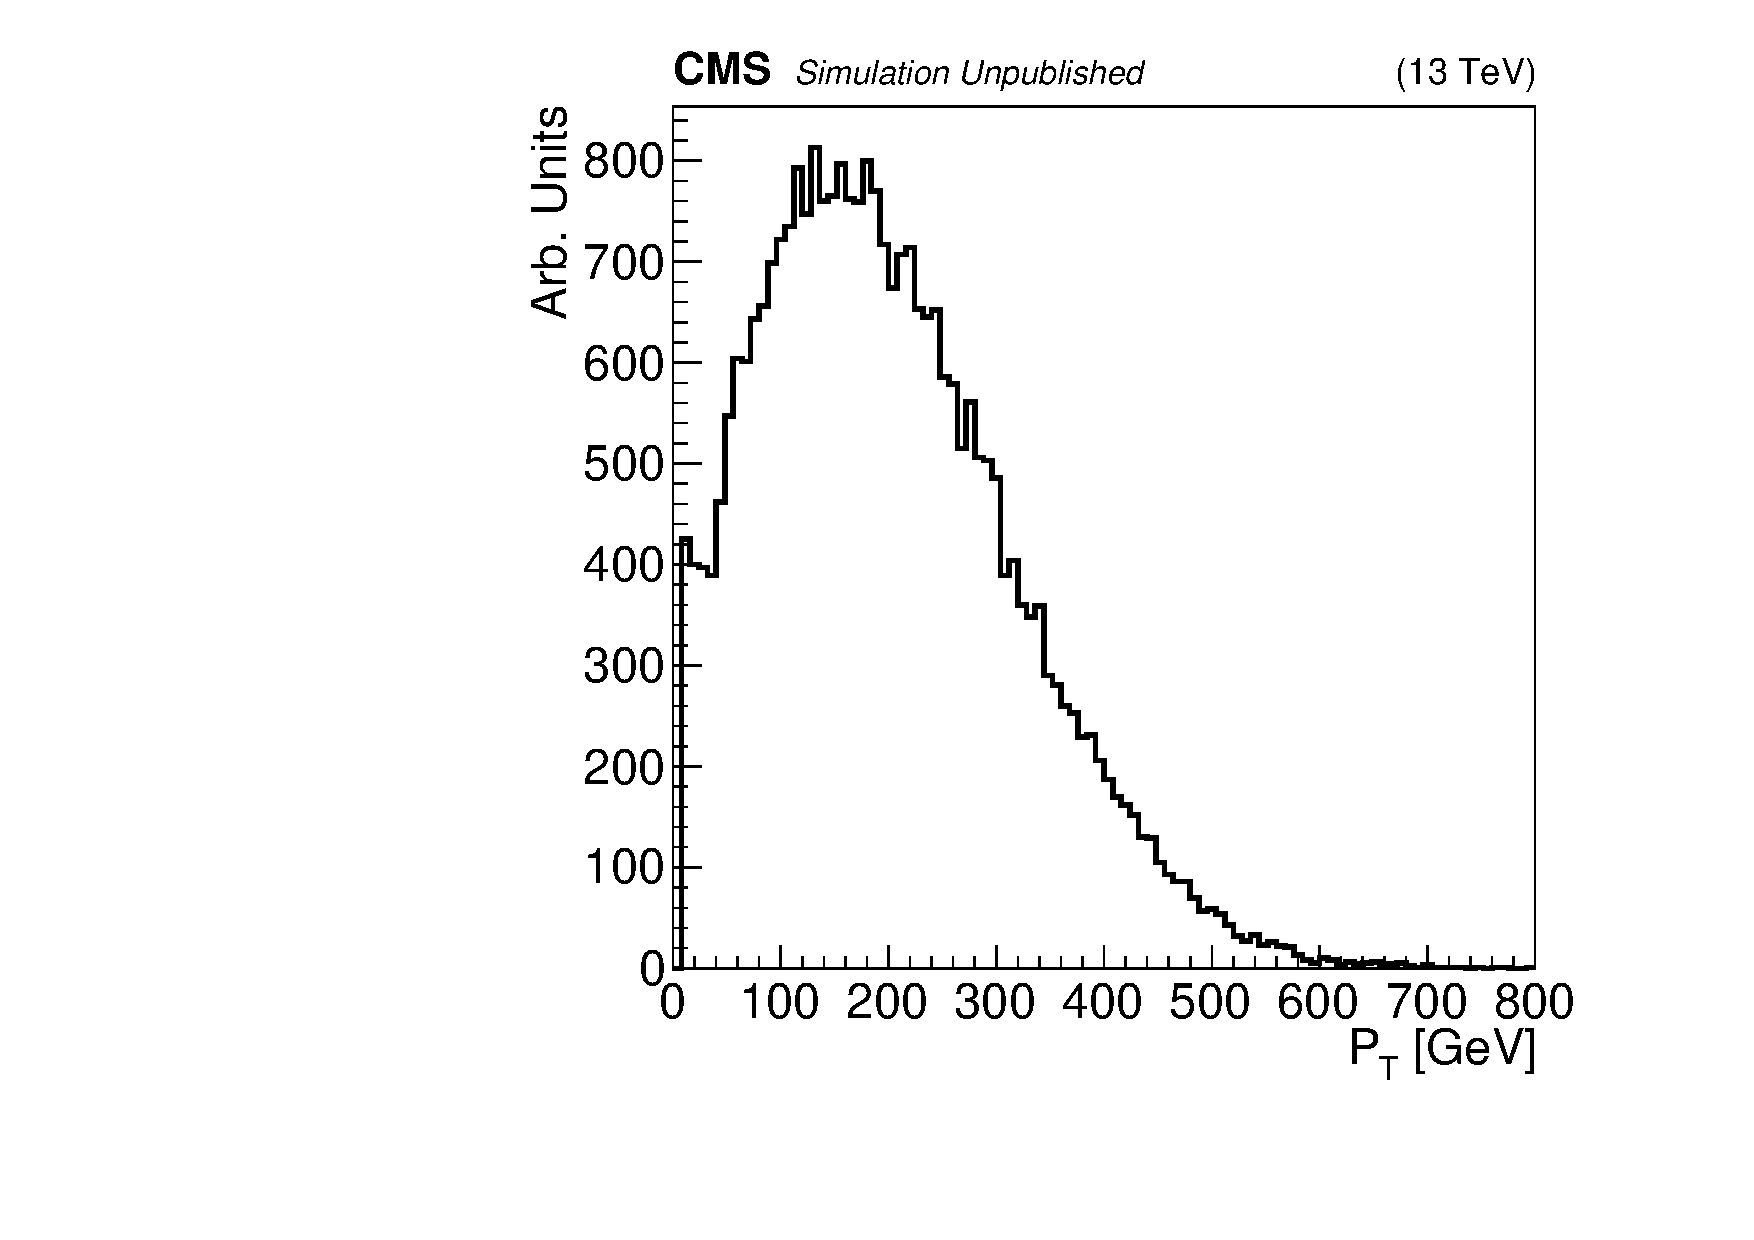
\includegraphics[width=2.4in]{figures/ptMatchedRecoJetTwo_mwr2200_mnu1100.pdf}
		\caption{jet from $\nul \rightarrow \ell jj$}\label{fig:wrLeptJetPtsd}
	\end{subfigure}
	\caption{The $\pt$ distributions of leptons and jets reconstructed in $\WR \rightarrow \ell\ell jj$ events with $\mWR = 2.2$ $\TeV$ 
		and $\mnul = \frac{1}{2}\mWR$.}\label{fig:wrLeptJetPts}
\end{figure}

\begin{figure}
	\centering
	\begin{subfigure}[t]{2.4in}
		\centering
		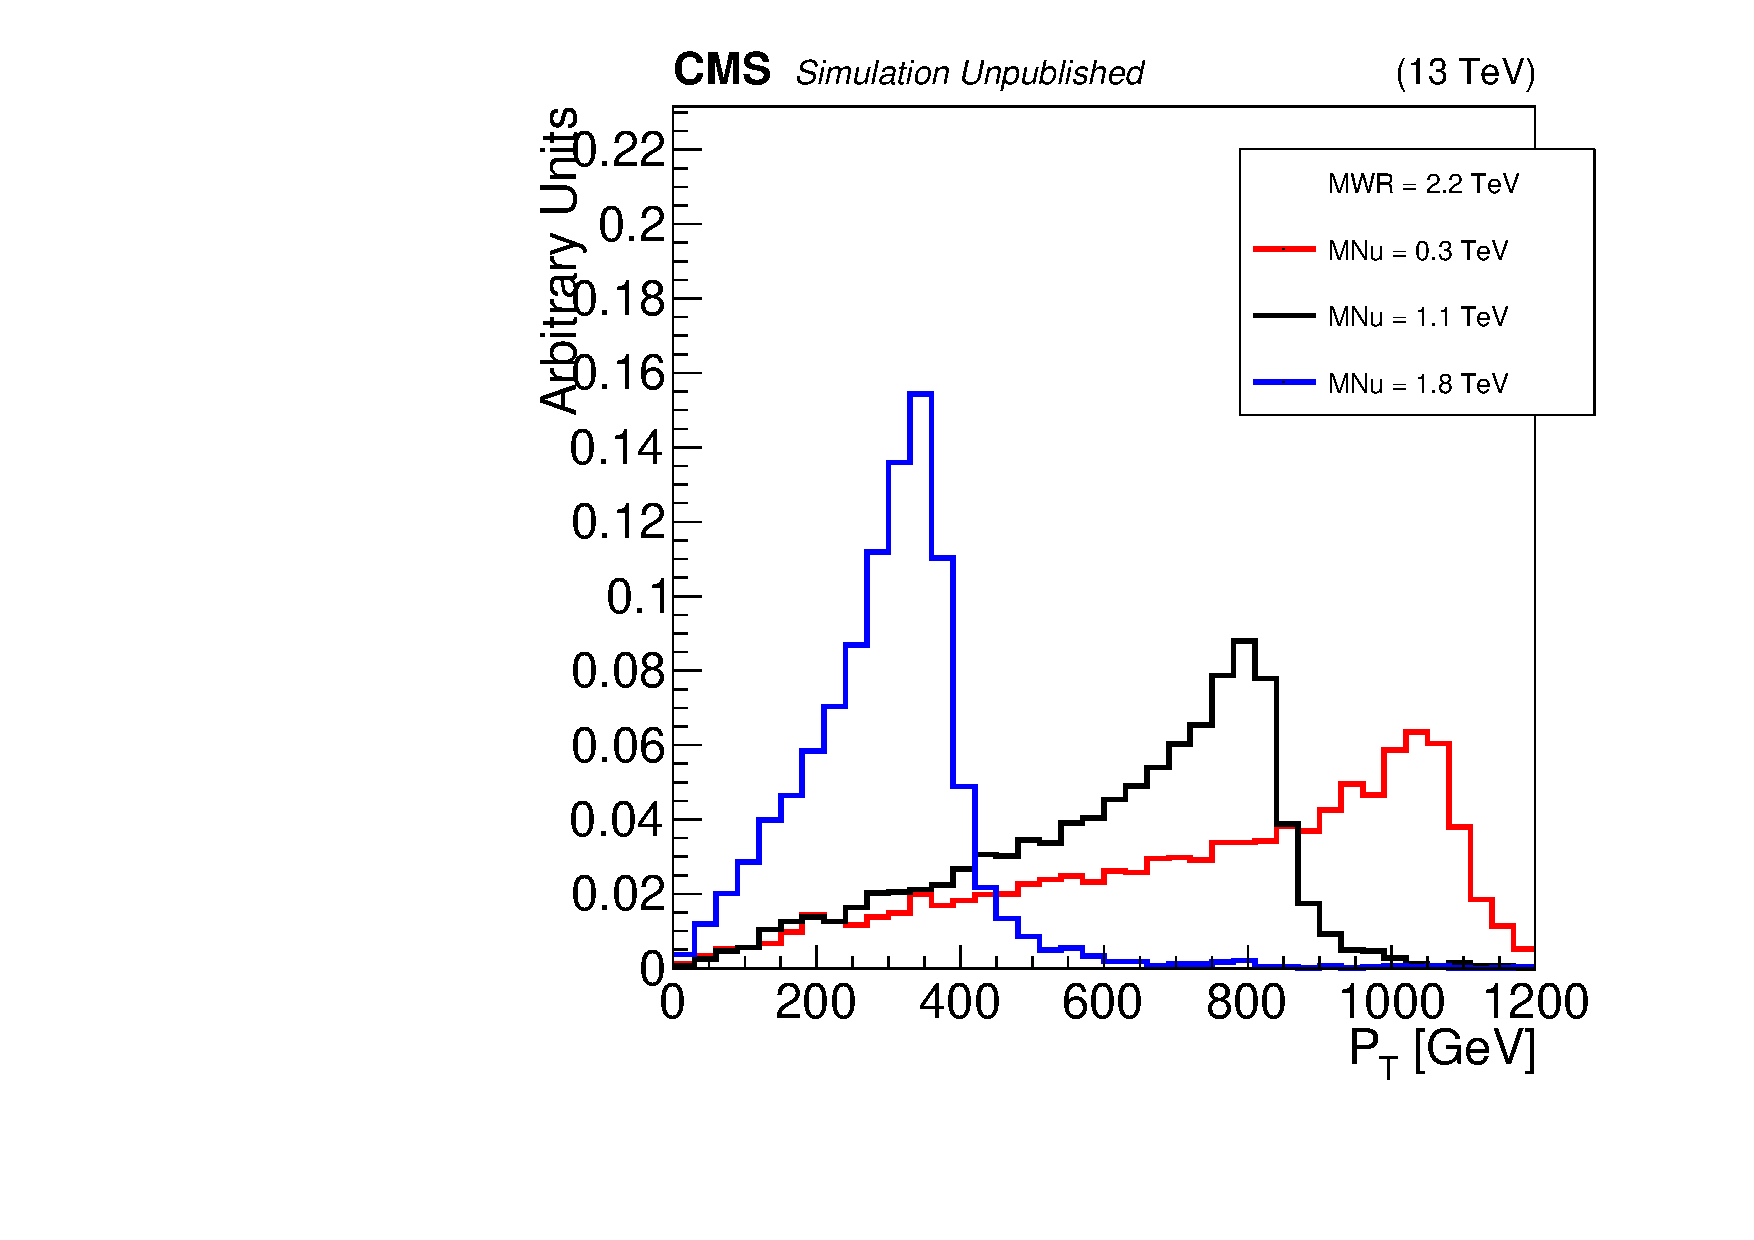
\includegraphics[width=2.4in]{figures/ptGenLeptFromFstHvyPtcl_MWR_2200_several_MNu_private.pdf}
		\caption{$\ell$ from $\WR \rightarrow \ell\nul$}\label{fig:wrLeptQrkPtsVarMNua}
	\end{subfigure}
	\thickspace
	\begin{subfigure}[t]{2.4in}
		\centering
		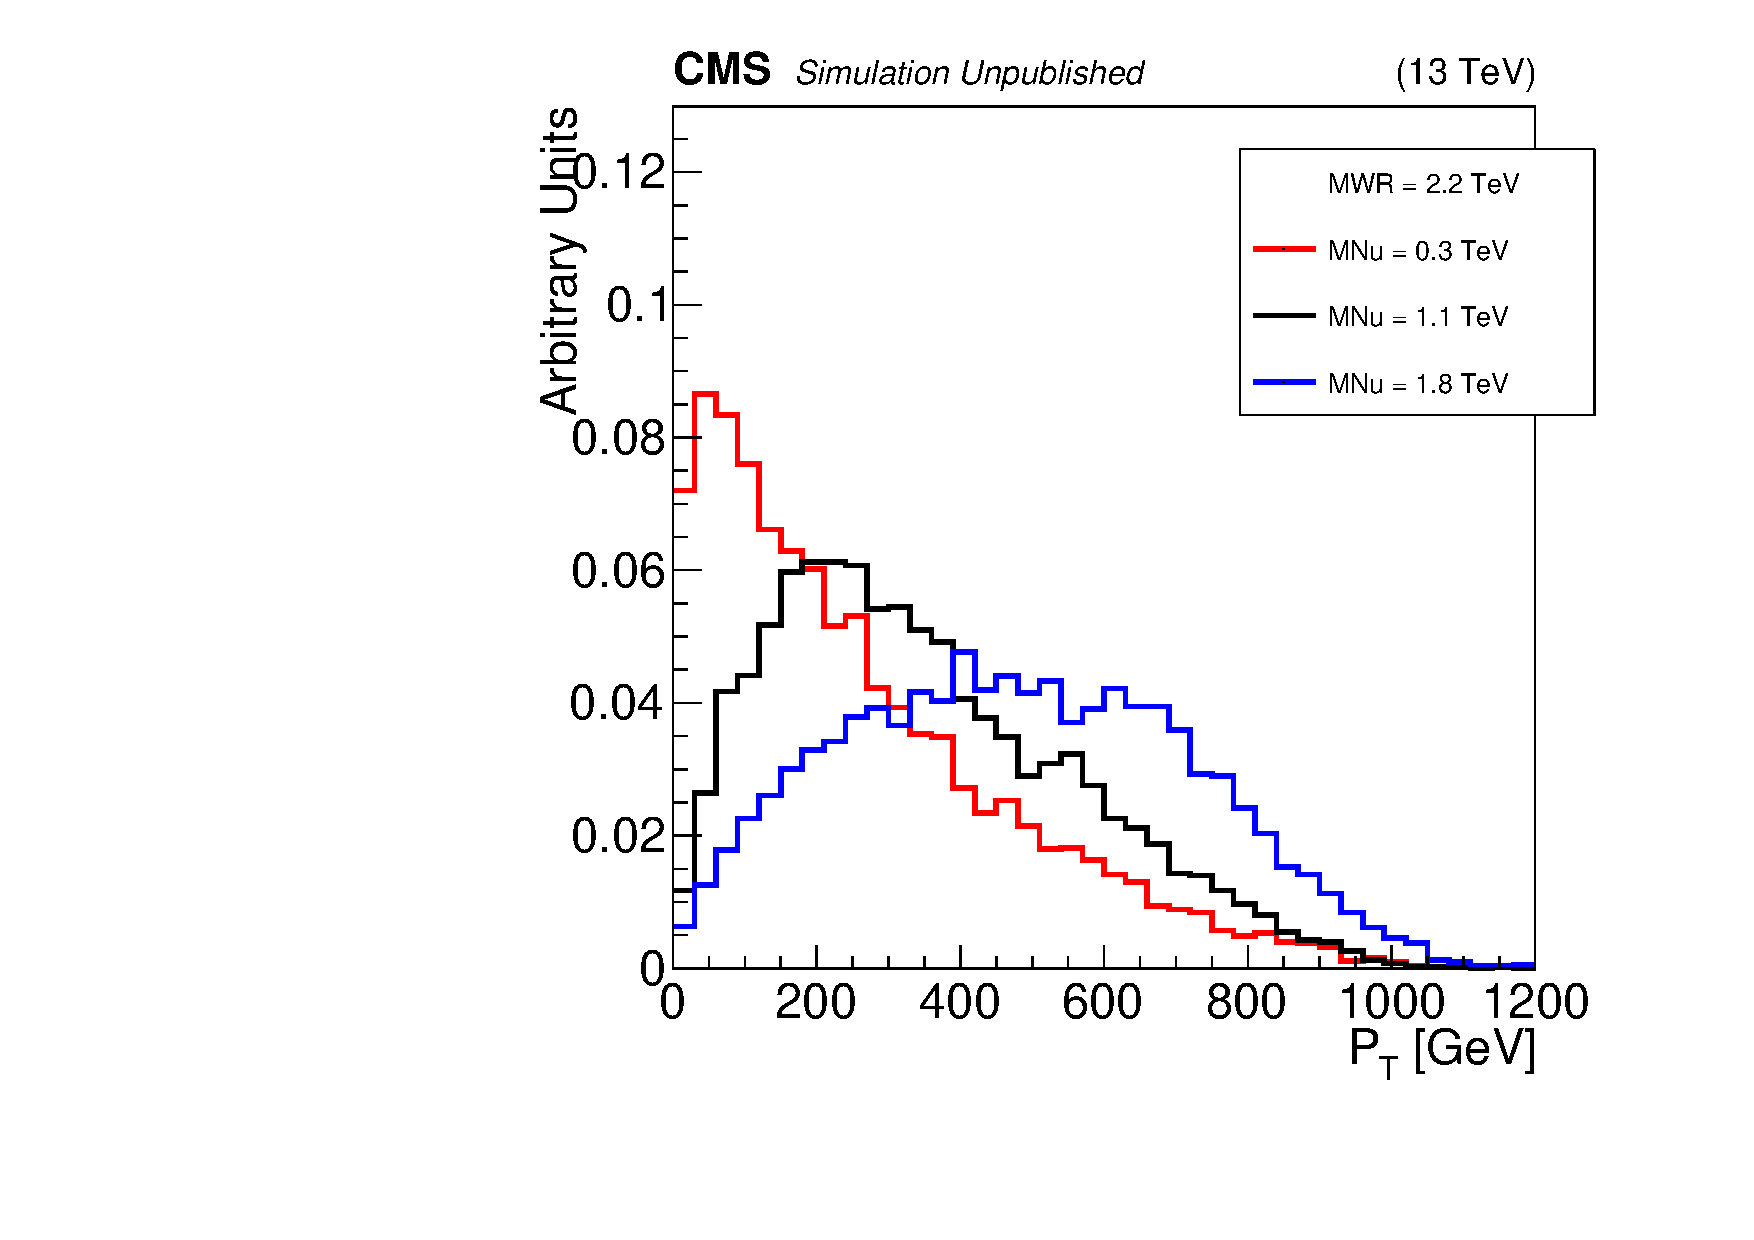
\includegraphics[width=2.4in]{figures/ptGenLeptFromScdHvyPtcl_MWR_2200_several_MNu_private.pdf}
		\caption{$\ell$ from $\nul \rightarrow \ell qq$}\label{fig:wrLeptQrkPtsVarMNub}
	\end{subfigure}
	\newline
	\newline
	\newline
	\newline
	\begin{subfigure}[t]{2.4in}
		\centering
		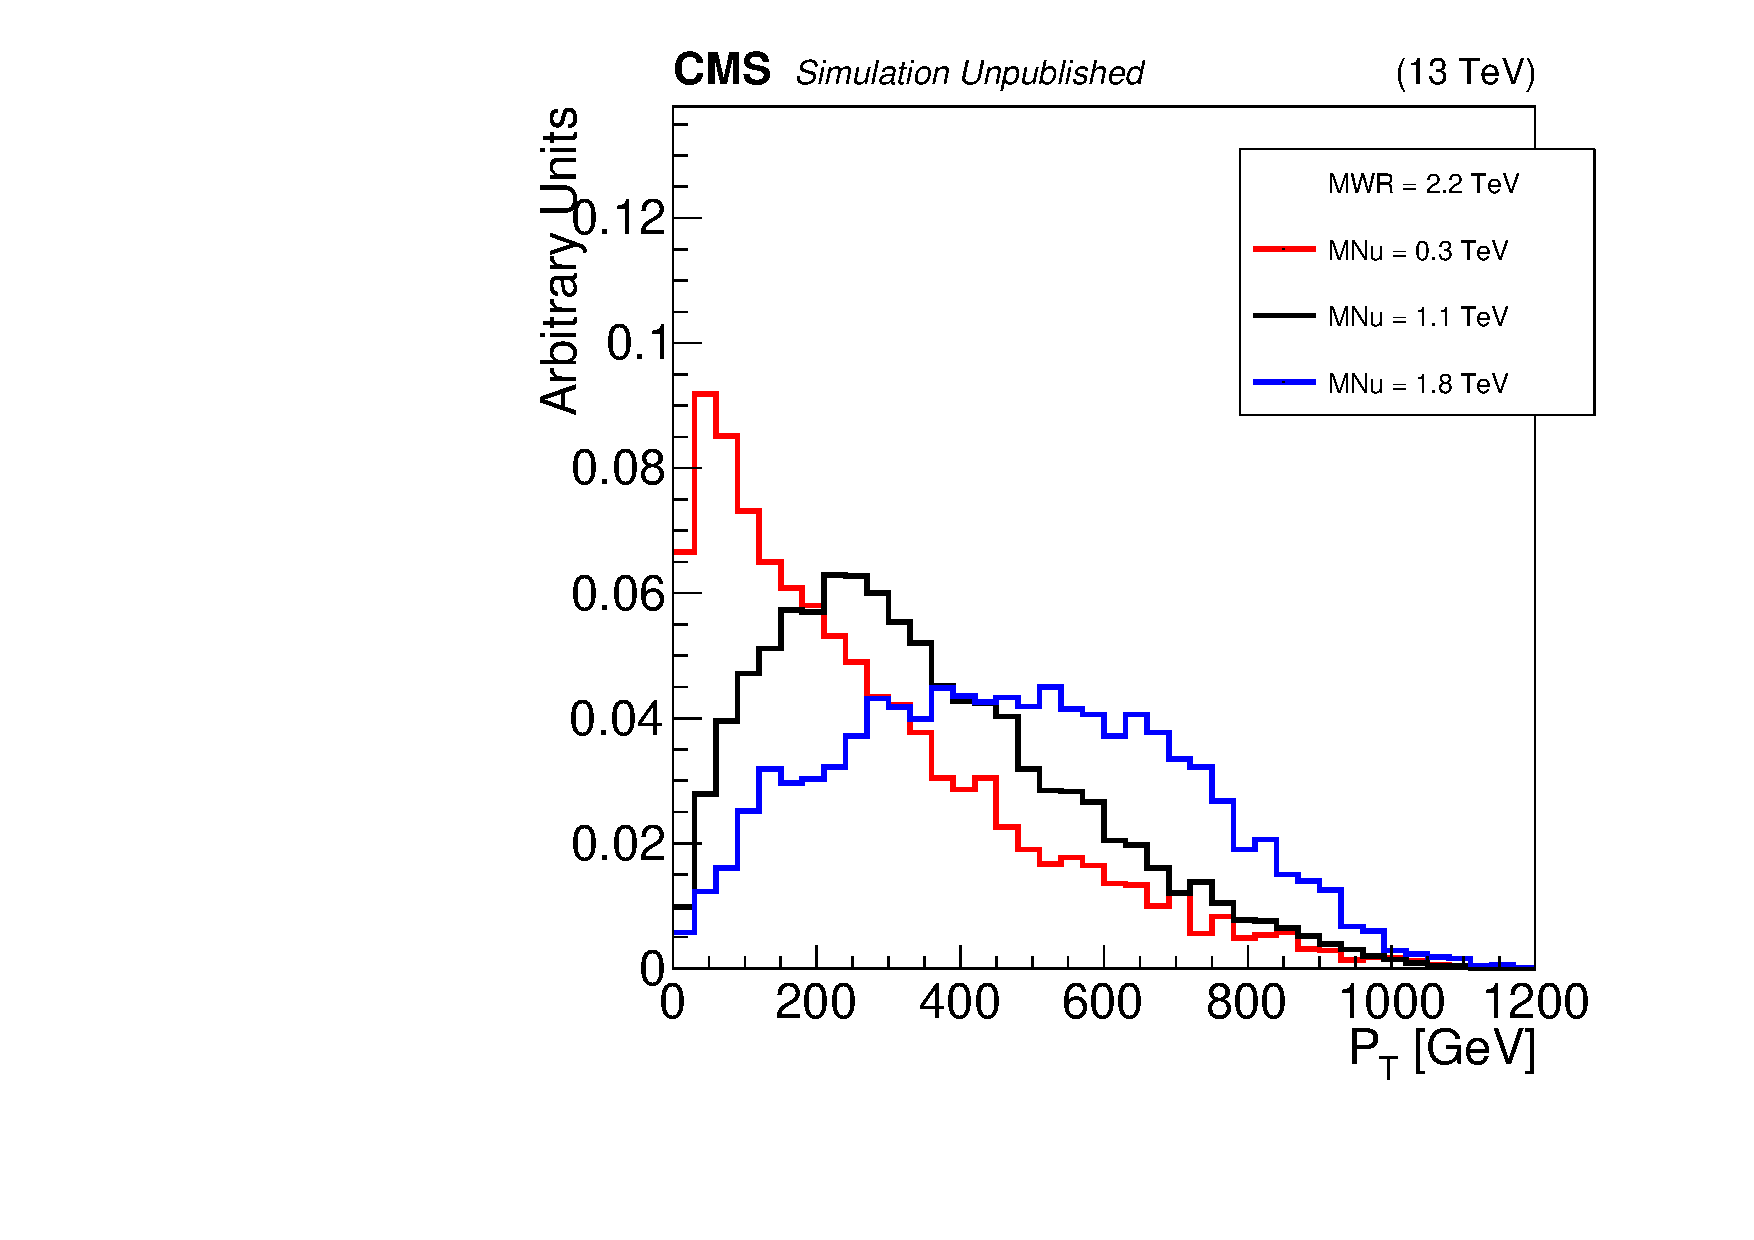
\includegraphics[width=2.4in]{figures/ptGenQuarkOneFromScdHvyPtcl_MWR_2200_several_MNu_private.pdf}
		\caption{quark from $\nul \rightarrow \ell qq$}\label{fig:wrLeptQrkPtsVarMNuc}
	\end{subfigure}
	\thickspace
	\begin{subfigure}[t]{2.4in}
		\centering
		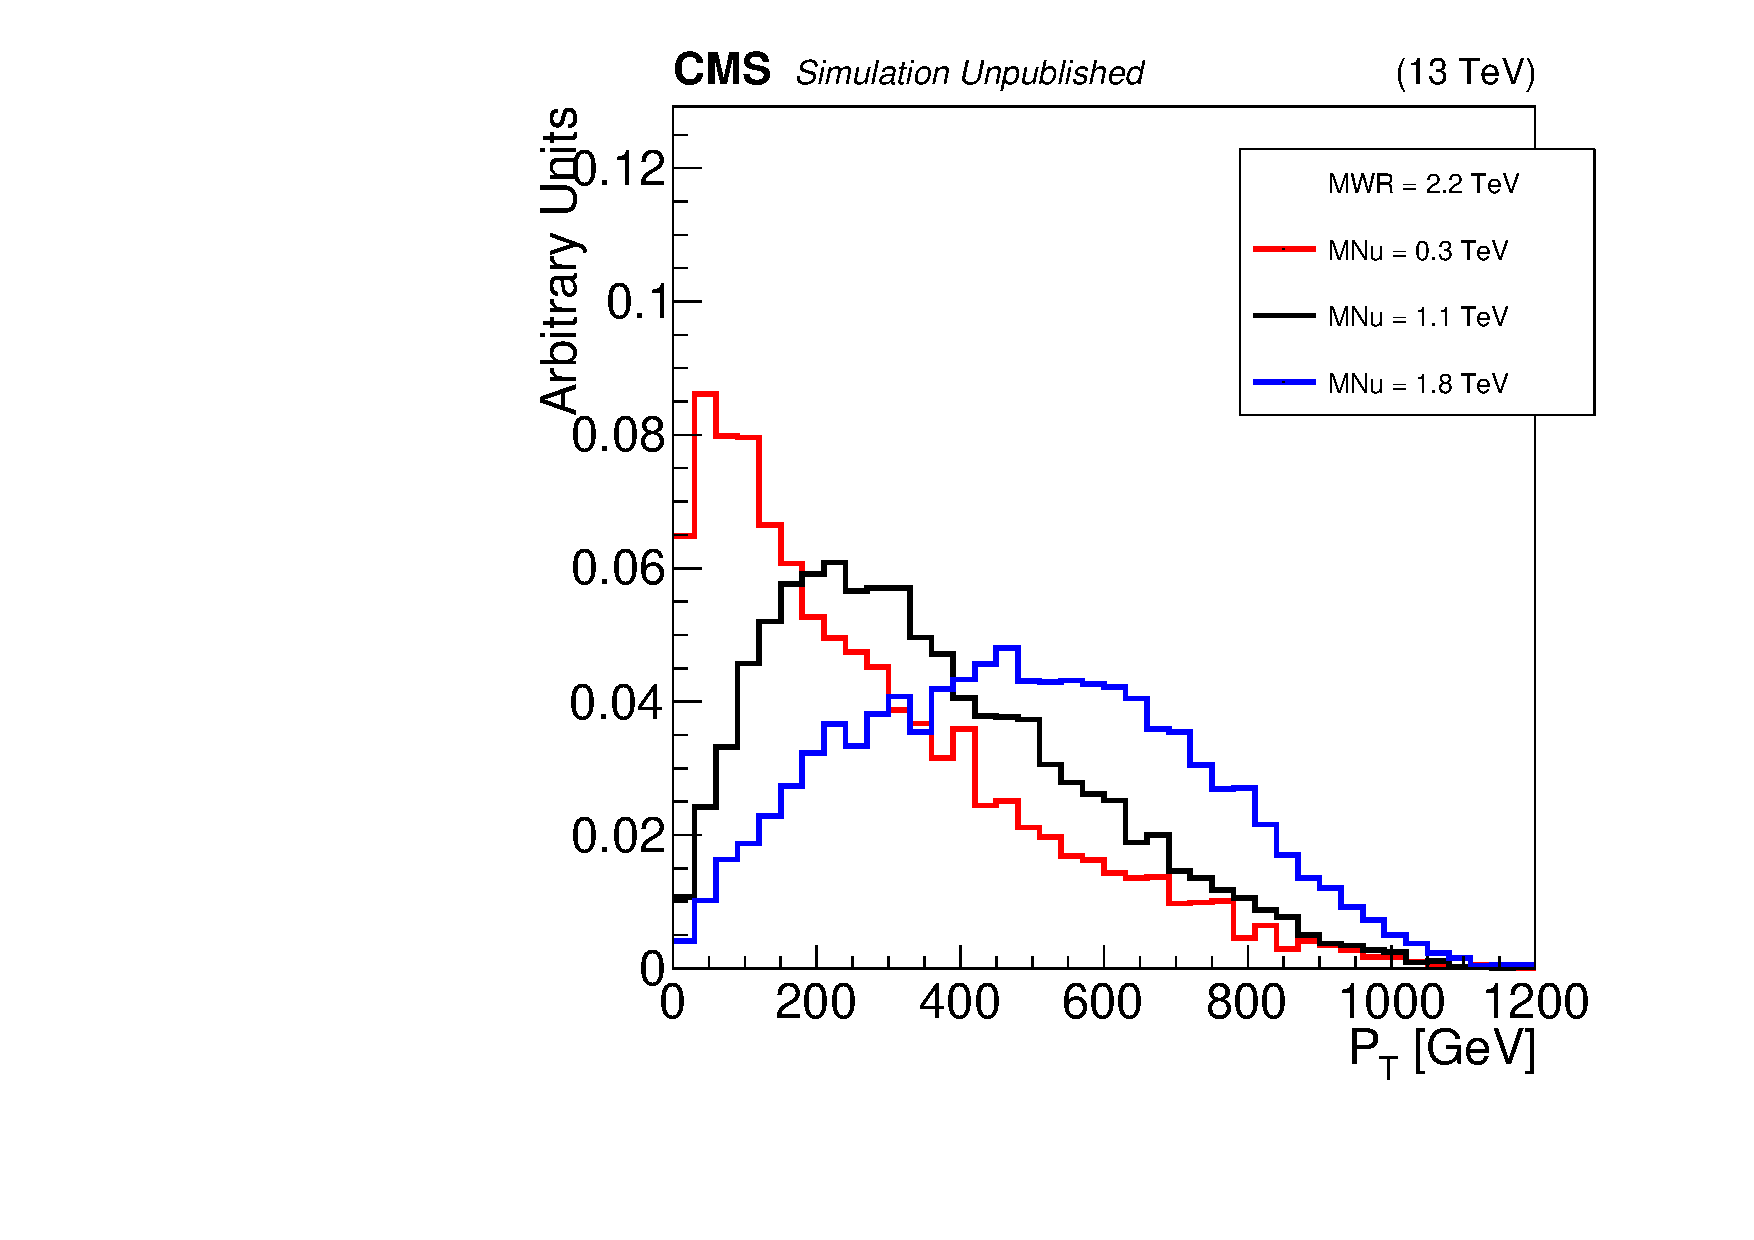
\includegraphics[width=2.4in]{figures/ptGenQuarkTwoFromScdHvyPtcl_MWR_2200_several_MNu_private.pdf}
		\caption{quark from $\nul \rightarrow \ell qq$}\label{fig:wrLeptQrkPtsVarMNud}
	\end{subfigure}
	\caption{The $\pt$ distributions of leptons and quarks produced in $\WR \rightarrow \ell\ell qq$ events with $\mWR = 2.2$ $\TeV$ 
		and different \mnul.}\label{fig:wrLeptQrkPtsVarMNu}
\end{figure}
\clearpage

Based on these kinematics, one reconstructed lepton was required to have $\pt > 60$ $\GeV$, and the other $\pt$ selection criteria 
were as low as possible to increase sensitivity to \WR signals with low $\mnul/\mWR$.  The jet $\pt$ requirement was 
set based on the decrease in jet $\pt$ resolution with jet $\pt$.  For reconstructed jets that were measured in the region $|\eta| < 1.3$, 
the jet $\pt$ resolution was 16\% of $\pt$ or better for $\pt > 40$ $\GeV$, and $\sim$21\% of $\pt$ for $30 < \pt < 40$ $\GeV$ 
\cite{jetResolutionInCollisions}.  The two selected jets were required to have $\pt > 40$ $\GeV$ to avoid selecting low $\pt$ jets that 
were measured with poor $\pt$ resolution.  The $\pt$ selection criterion applied to the lower $\pt$ reconstructed lepton was set based on 
the lepton trigger selection efficiency.  These efficiencies as a function of reconstructed muon and electron $\pt$, shown in Figure 
\ref{fig:trigEffs}, are constant for $\pt > 53$ $\GeV$, so the second reconstructed lepton was required to have $\pt > 53$ $\GeV$.

\begin{figure}
	\centering
	\begin{subfigure}[t]{2.4in}
		\centering
		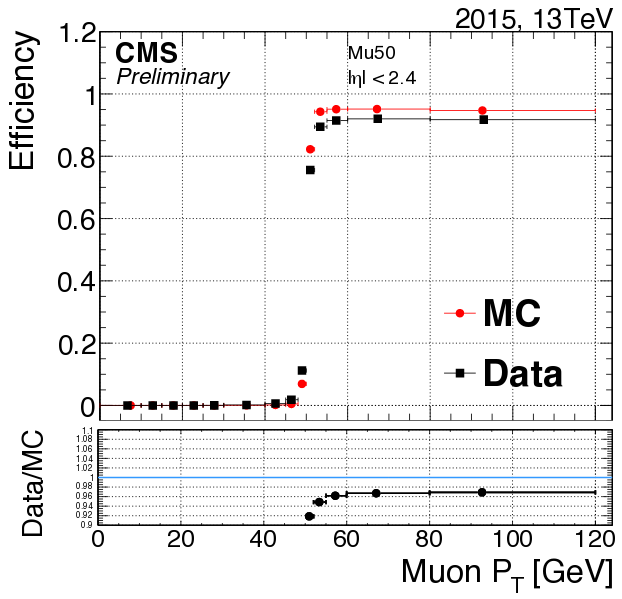
\includegraphics[width=2.4in]{figures/muonPt50TrgEffVsPt.png}
		%\caption{muon}\label{fig:trigEffsa}
	\end{subfigure}
	\newline
	\newline
	\newline
	\newline
	\begin{subfigure}[t]{2.4in}
		\centering
		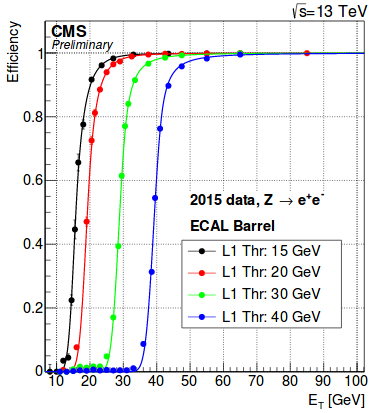
\includegraphics[width=2.4in]{figures/L1EGEfficiencyBarrel.png}
		%\caption{barrel electron}\label{fig:trigEffsb}
	\end{subfigure}
	\thickspace
	\begin{subfigure}[t]{2.4in}
		\centering
		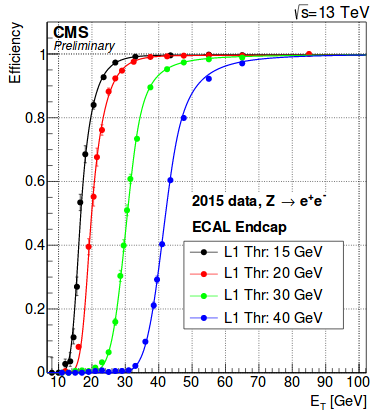
\includegraphics[width=2.4in]{figures/L1EGEfficiencyEndcap.png}
		%\caption{endcap electron}\label{fig:trigEffsc}
	\end{subfigure}
	\caption{The muon and electron trigger efficiencies as a function of $\pt$ or $\Et$ in $Z \rightarrow \ell\ell$ events.}\label{fig:trigEffs}
\end{figure}
\clearpage

The invariant mass of the two leptons ($\Mll$), given by Equation \ref{eq:dileptMass}, is affected by the \WR mass and the ratio $\mnul/\mWR$.  
As the \WR mass increases the $\pt$ of both leptons also increase, thus increasing the $\Mll$.  At a fixed \WR mass the ratio $\mnul/\mWR$ 
affects the $\Mll$ as follows.  In the decay $\WR \rightarrow \ell_{1}\nul$, the \nul always recoils against $\ell_{1}$.  As $\mnul/\mWR$ 
decreases to 0 the $\ell_{2}$ from the decay $\nul \rightarrow \ell_{2} jj$ is increasingly boosted along the \nul direction of momentum, 
and opposite to the $\ell_{1}$ direction of momentum.  Therefore, as $\mnul/\mWR$ decreases the angle $\theta_{12}$ between the two leptons, 
shown in Figure \ref{fig:wrLeptAngleSepVarMNu}, increases, and the $\Mll$ increases, as shown in Figure \ref{fig:wrMllVarMNu}.  Based on 
the large expected \WR mass, the two reconstructed leptons were required to have $\Mll > 200$ $\GeV$.  The $\Mll$ threshold was not increased 
because it would reduce sensitivity to \WR signals with $\mnul/\mWR \sim$1; the threshold was not lowered because it would increase 
backgrounds, especially from $\DY$+jets production, without a corresponding increase in the signal.

\begin{equation}
	\Mll = \sqrt{2|p_{1}||p_{2}|(1\thickspace - \thickspace \cos(\theta_{12}))}
	\label{eq:dileptMass}
\end{equation}

\begin{figure}[h]
	\centering
	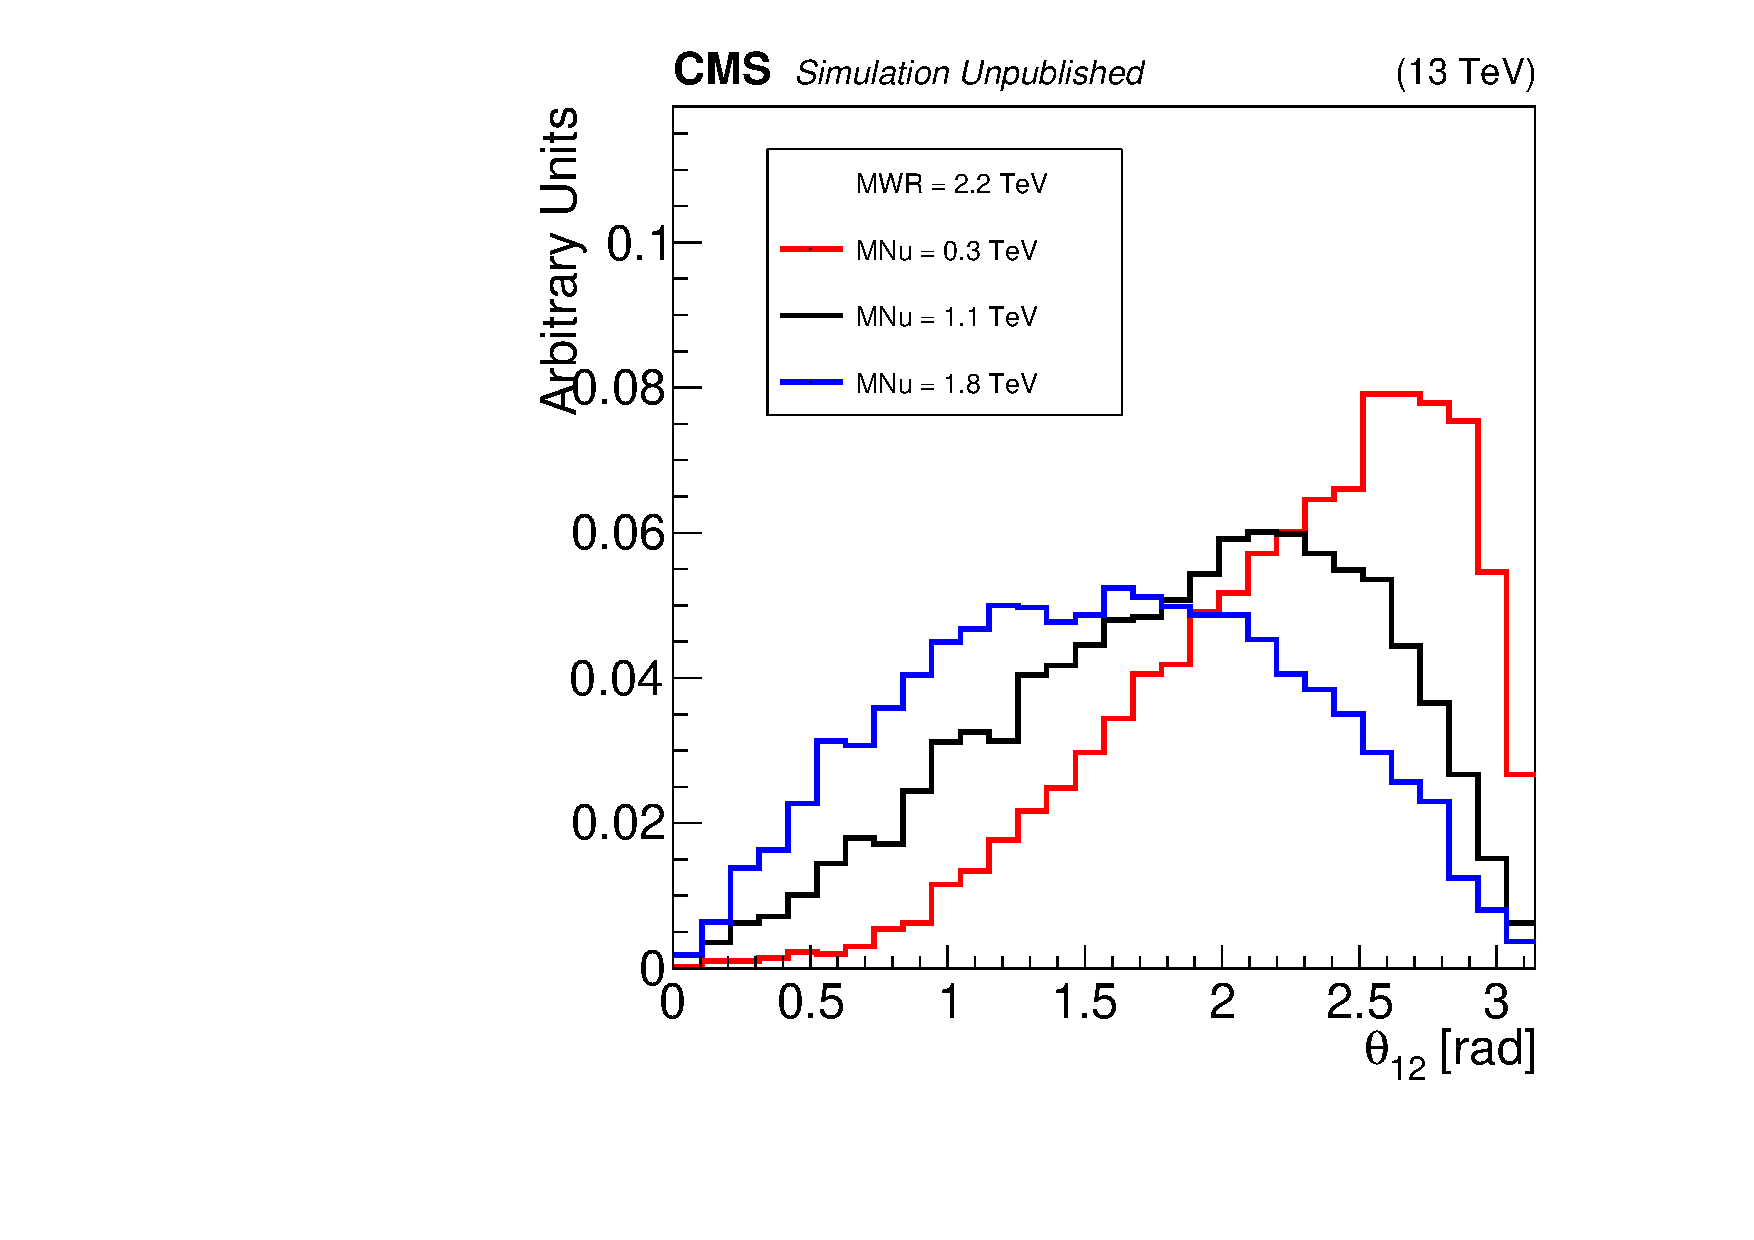
\includegraphics[width=0.5\textwidth]{figures/angleBtwnGenLepts_MWR_2200_several_MNu_private.pdf}
	\caption{The distribution of the angle $\theta_{12}$ between the two leptons produced in $\WR \rightarrow \ell_{1}\ell_{2} qq$ events with 
		$\mWR = 2.2$ $\TeV$ and different \mnul.}
	\label{fig:wrLeptAngleSepVarMNu}
\end{figure}

\begin{figure}[h]
	\centering
	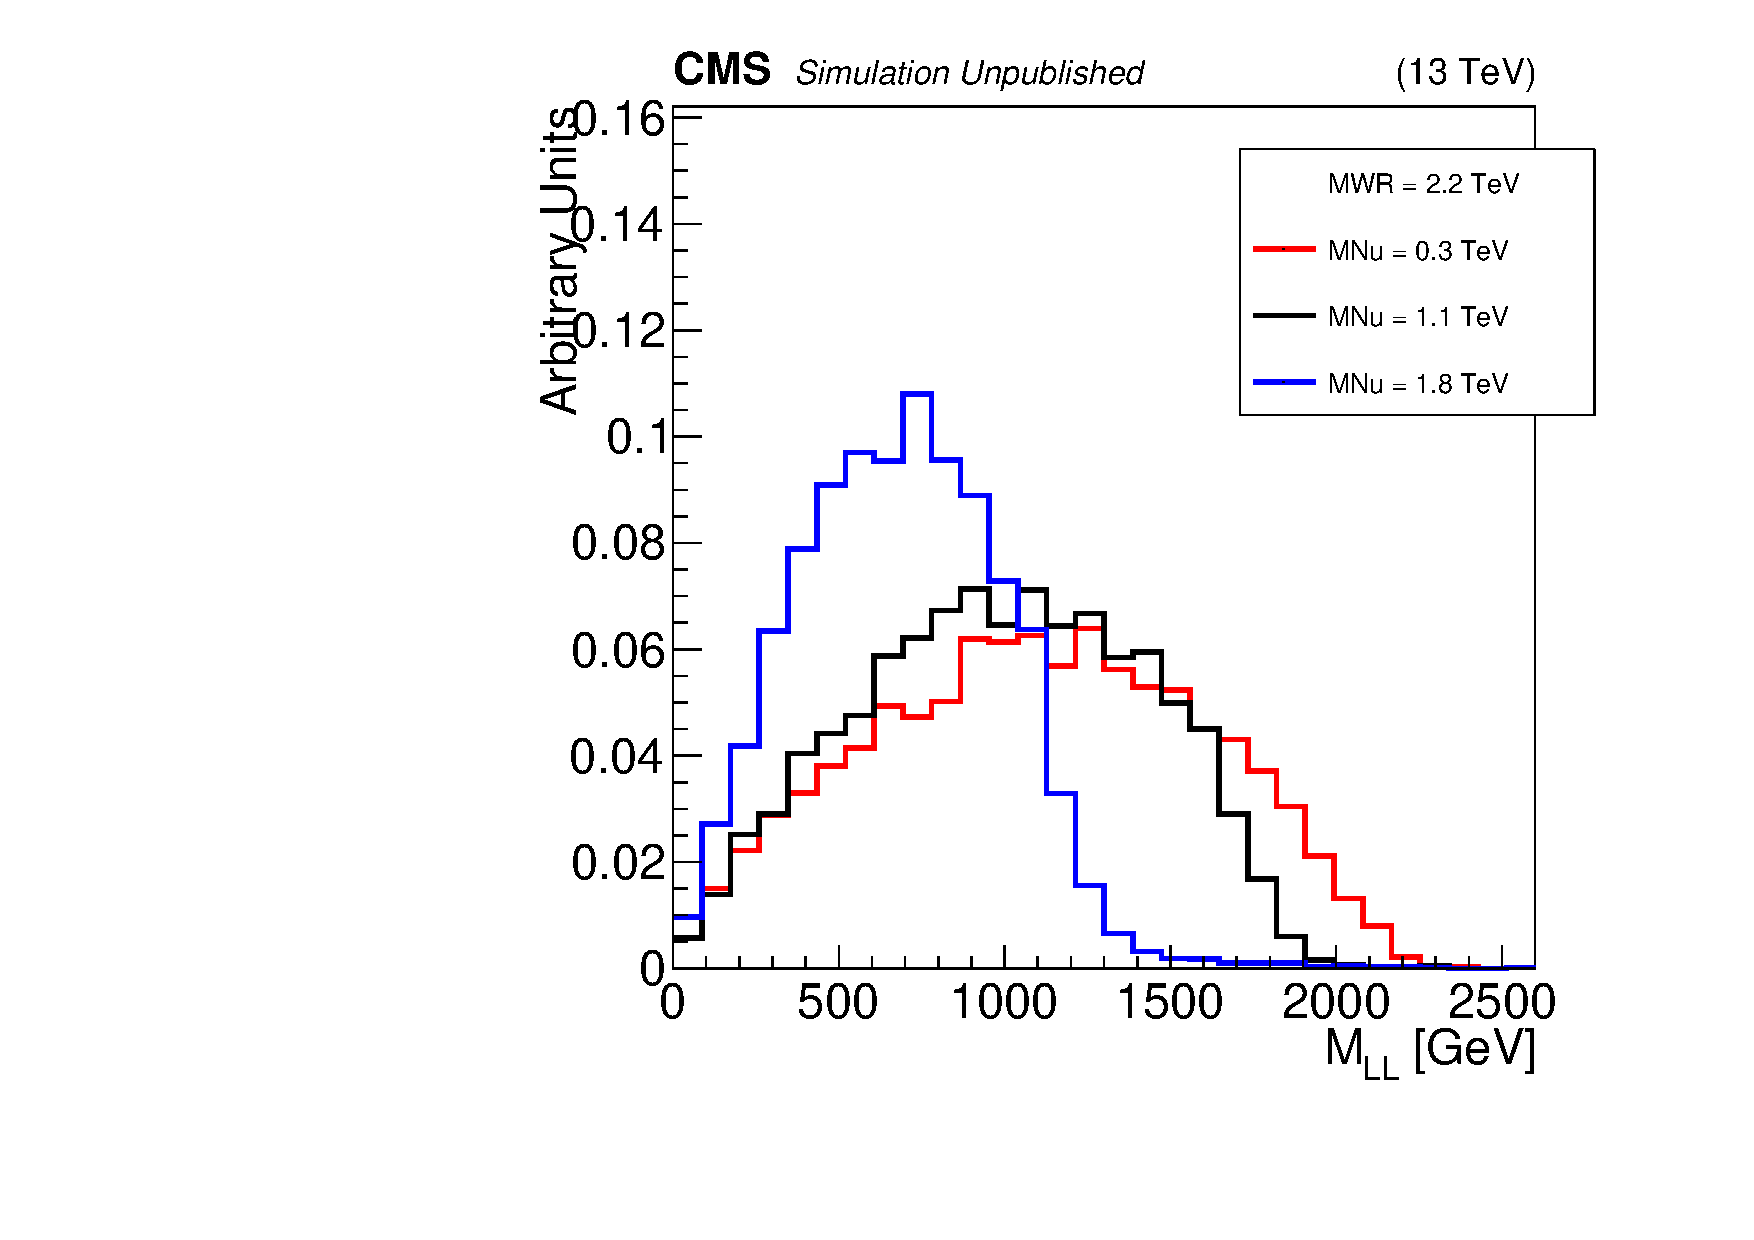
\includegraphics[width=0.5\textwidth]{figures/dileptonMassFromGenLeptonsFromFstAndScdHvyPtcl_MWR_2200_several_MNu_private.pdf}
	\caption{The $\Mll$ distribution of the two leptons produced in $\WR \rightarrow \ell\ell qq$ events with $\mWR = 2.2$ $\TeV$ and 
	different \mnul.}
	\label{fig:wrMllVarMNu}
\end{figure}
\clearpage

In selected events, if more than two jets passed the selection criteria described previously, the two highest $\pt$ jets were selected.

Applying the selection criteria described previously to simulated ST background events created a peak in the $\Mlljj$ distribution 
near 500 $\GeV$, as shown in Figure \ref{fig:sculptedMlljj}.  To avoid this peak, each event was required to have $\Mlljj > 600$ $\GeV$.

\begin{figure}[h]
	\centering
	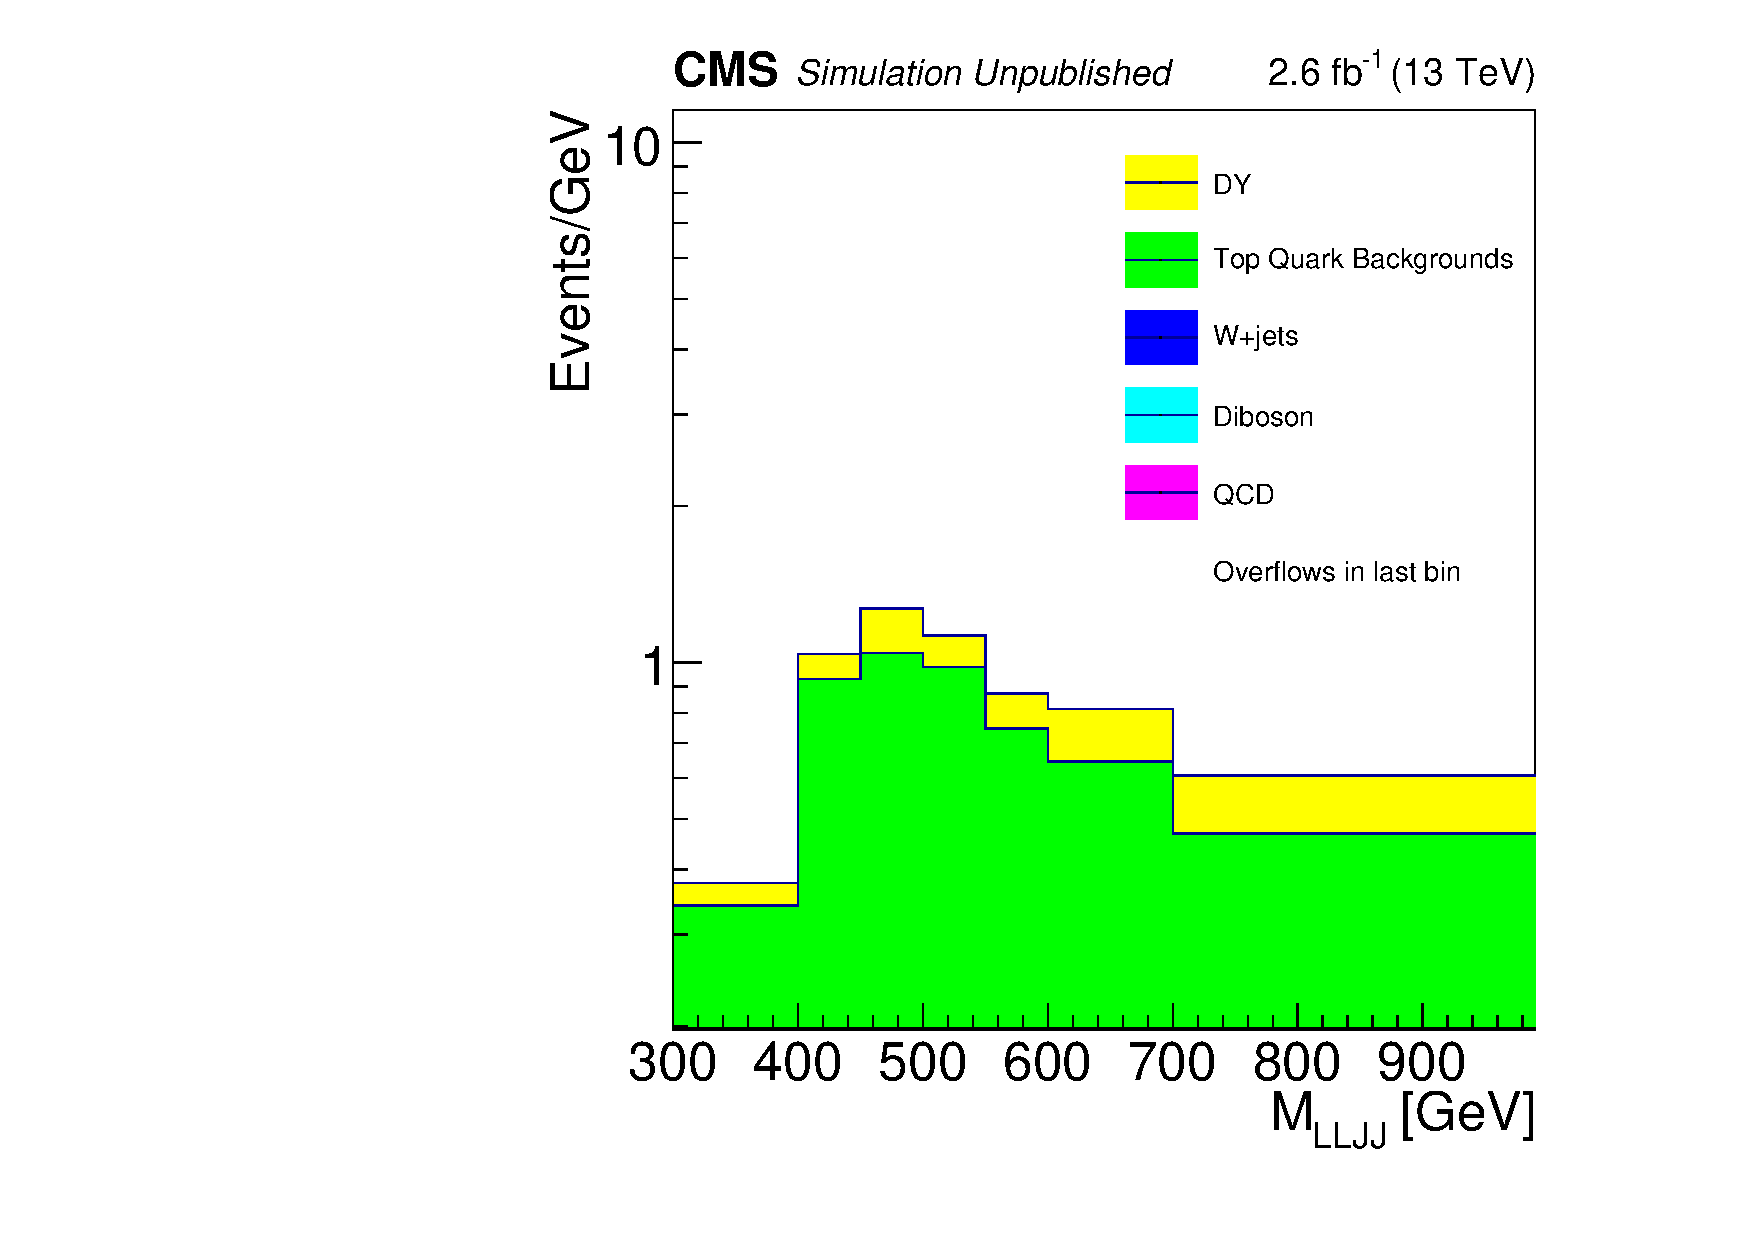
\includegraphics[width=0.45\textwidth]{figures/Mlljj_varBins_SignalRegion_EEChannelBkgndMC_DYMadHTAndIncl_TTBarFromData_log.pdf}
	\caption{The $\Mlljj$ distribution in simulated background events after applying the event selection.}
	\label{fig:sculptedMlljj}
\end{figure}
\clearpage

The offline kinematic selection criteria, listed in Table \ref{tab:offlineKinemSel}, were developed to select $\WR \rightarrow \ell\ell jj$ 
events over a large range of \mWR and \mnul values with the highest possible efficiency.  The efficiency of the event selection, 
including trigger selection criteria, in signal events was estimated by simulating $pp \rightarrow \WR \rightarrow \ell\ell jj$ 
interactions, and applying the event selection to those events.  The \PYTHIA \MC generator implements a flexible, generic \WR signal 
model that captures the main characteristics of theoretical models discussed in the literature 
\cite{earlyLRSModel,lrsHiggsStageOne,lrsHiggsStageTwo,seeSawAndParityViolation,seeSawAndGUTs,lrsMassConstraints}, so \PYTHIA was used to 
simulate $\WR \rightarrow \ell\ell jj$ events with different values of \mWR and \mnul.  The event selection efficiency was calculated 
using 50000 event datasets produced with $\mnul = \frac{1}{2}\mWR$ and \mWR stepping from 0.8 to 6.0 $\TeV$ in increments of 0.2 $\TeV$.  
The event selection efficiency, shown in Figure \ref{fig:wrRecoSelectionEff}, exceeded 50\% in the $ee$-channel, and 70\% in the 
$\mu\mu$-channel.  The efficiency is lower in the $ee$-channel due to the gap in ECAL coverage for $1.44 < |\eta| < 1.57$, and the lower 
efficiency offline ID criteria applied to electrons relative to muons.

\begin{table}[h]
	\caption{The kinematic selection criteria applied to reconstructed leptons and jets.  The criteria were applied in the order 
	that they are listed.}
	\label{tab:offlineKinemSel}
	\centering
	\begin{tabular}{c|c}
		parameter & threshold  \\  \hline
		lead jet $\pt,\eta$ & $\pt>40\GeV,|\eta|<2.4$ \\
		sublead jet $\pt,\eta$ & $\pt>40\GeV,|\eta|<2.4$ \\
		lead $\ell$ $\pt,\eta$ & $\pt>60\GeV,|\eta|<2.4$ \\
		sublead $\ell$ $\pt,\eta$ & $\pt>53\GeV,|\eta|<2.4$ \\
		$\Delta R(\ell,j)$ & $>0.4$ \\
		$\Mll$ & $>200\GeV$ \\
		$\Mlljj$ & $>600\GeV$ \\ \hline
	\end{tabular}
\end{table}

\begin{figure}[h]
	\centering
	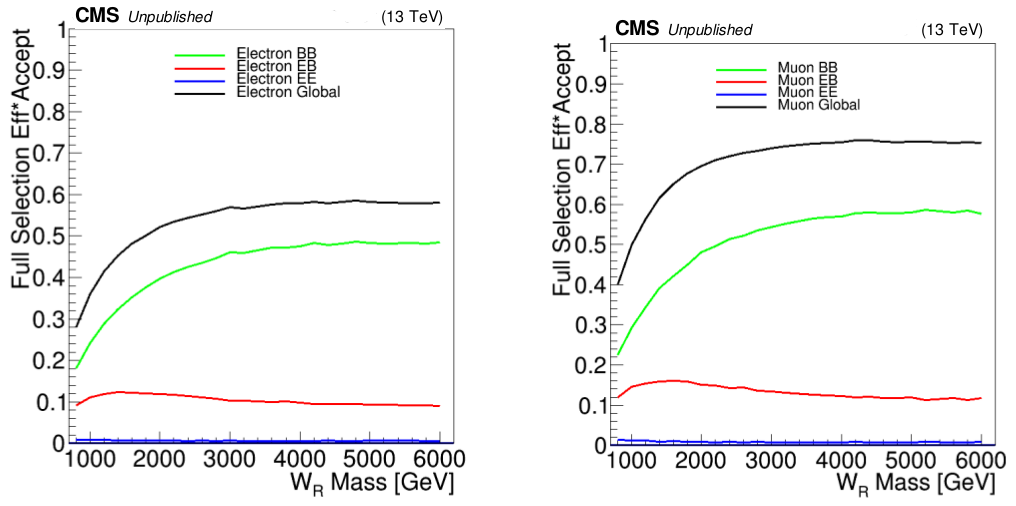
\includegraphics[width=1.0\textwidth]{figures/wrRecoSelectionEfficiency.png}
	\caption{The event selection efficiency in simulated $\WR \rightarrow \ell\ell jj$ events, in the $ee$-channel (left) and the 
		$\mu\mu$-channel (right).  Different curves represent events where both leptons are in the barrel (BB), one is in the 
	endcap (EB), or both are in the endcap (EE).}
	\label{fig:wrRecoSelectionEff}
\end{figure}
\clearpage

At a specific \WR mass, only the offline kinematic selection efficiency varied by more than a few percent over the entire \mnul range.  The 
variation in this selection efficiency as a function of \mnul was calculated using 10000 event datasets produced with \mWR increasing 
from 0.8 to 4.0 $\TeV$ in increments of 0.1 $\TeV$.  At each \WR mass, 10000 events were produced at each value of \mnul starting at 
100 $\GeV$ and increasing to \mWR in increments of 0.1 $\TeV$ or less.  The maximum variation in the kinematic selection efficiency as a 
function of \mnul, shown in Figure \ref{fig:wrOffSelEffVarMWrMNu}, increased with \mWR: up to 30\% for $\mWR \leq 1.3$ $\TeV$, and up 
to 70\% for $\mWR \geq 2.5$ $\TeV$.  At a specific \WR mass, the kinematic selection efficiency is maximized or nearly so when 
$\mnul = \frac{1}{2}\mWR$.

\begin{figure}[h]
	\centering
	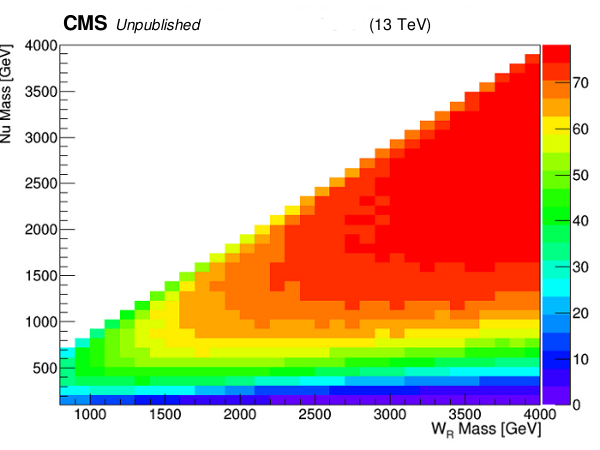
\includegraphics[width=1.0\textwidth]{figures/genWrMuMuAccEff_NoMassWindows13TeV.png}
	\caption{The offline kinematic selection efficiency (\%) in $\WR \rightarrow \ell\ell jj$ events as a function of \mWR and \mnul.}
	\label{fig:wrOffSelEffVarMWrMNu}
\end{figure}
\clearpage

\section{Reconstruction and Event Selection Summary}
\label{sec:recoConclusion}
Electrons, muons and jets expected from \WR and \nul decays are reconstructed from signals measured in CMS sub-detectors using dedicated 
reconstruction algorithms.  These algorithms reconstruct leptons, hadrons and jets with high efficiency by using minimal selection criteria, 
and occasionally ($\sim$1-3\%) reconstruct individual particles and jets incorrectly.  The contribution of incorrectly 
reconstructed particles to $\ell\ell jj$ events was reduced by selecting events using lepton triggers and requiring that leptons and jets 
were reconstructed from high quality measurements.  
Selected particles were then required to pass kinematic selection criteria to identify particles whose kinematics are consistent with the 
\WR progeny.  After applying the event selection to the data, the selected events were used to make a $\Mlljj$ distribution.  The decay 
$\WR \rightarrow \ell\ell jj$ transfers all energy of the \WR into the invariant mass of the leptons and jets, so evidence of a \WR, 
independent of \mnul, was searched for as an excess of data events above the predicted background in the $\Mlljj$ distribution.  The 
contribution of background processes to the $\Mlljj$ distribution found in the data was predicted using procedures described in the next 
chapter.

%%%%%%%%%%%%%%%%%%%%%%%%%%%%%%%%%%%%%%%%%%%%%%%%%%%%%%%%%%%%%%%%%%%%%%%%%%%%%%%%
